\documentclass[review,hidelinks,onefignum,onetabnum]{siamonline250211}
% V13 public preprint; earlier published editions remain preserved.
\usepackage{microtype,xurl,needspace}
\usepackage{amsfonts,amssymb,mathtools,bm}
\usepackage{graphicx,booktabs,enumitem,float,tabularx,placeins,tikz}
\graphicspath{{./}{../siam-language-revision/}}
\usepackage[numbers,sort&compress]{natbib}
\newsiamremark{assumption}{Assumption}
\newsiamremark{remark}{Remark}
\headers{When Can Markets Crash Without News?}{Siyuan Ye}
\title{When Can Markets Crash Without News?}
\author{Siyuan Ye\thanks{Independent Researcher.}}
\hypersetup{pdftitle={When Can Markets Crash Without News?},pdfauthor={Siyuan Ye}}
\setlength{\emergencystretch}{1em}
% The unmodified online class's two-line running head exceeds its 10pt preset.
\setlength{\headheight}{14pt}
\newcommand{\R}{\mathbb{R}}
\newcommand{\Cris}{\mathcal{C}}
\newcommand{\calK}{\mathcal{K}}
\newcommand{\calA}{\mathcal{A}}
\newcommand{\dd}{\,\mathrm{d}}
\newcommand{\one}{\mathbf{1}}
\newcommand{\pos}[1]{[#1]_+}
\newcommand{\Law}{\mathcal{L}}
\newcommand{\totv}{\operatorname{TV}}
\renewcommand{\footercopyright}{}

\begin{document}
\raggedbottom
\maketitle
\begin{abstract}
Severe systemic price declines can be generated by admissible trading in an idealized multiasset market with fixed fundamentals, resilient price impact, paired-dollar execution, and zero terminal executed-dollar balances. A response-adapted price coordinate makes executed-dollar transfers additive, exposing a conservation law during trading and its interaction with recovery. We construct ten-asset paths in which all prices finish $50\%$ below their benchmarks and, separately, nine assets incur arbitrarily severe logarithmic losses under severity-independent finite turnover and inventory bounds. Under uniform $\pm25\%$ rolling price bands, a finite-rate path achieves two successive lower-limit closes for five assets, while a necessary bound excludes eight or more such closes; the maximal attainable coverage is unresolved. The certified path yields a $43.75\%$ target-asset loss and a geometric-index decline exceeding $16\%$. Elasticity barriers, a sharp full-coverage horizon bound, and execution-resource inequalities delimit these constructions.

\end{abstract}

\begin{keywords}market crashes; price impact; market resilience; systemic drawdown; reachability; execution constraints.\end{keywords}
\begin{MSCcodes}91G15, 91G45, 93B03, 65G30, 91G80.\end{MSCcodes}

\section{Introduction}\label{sec:intro}
Large market declines are commonly associated with adverse news, but transactions can change prices even when fundamentals remain fixed. This raises a basic question: can trading paths obeying a market's execution rules generate a severe, broad price decline without a negative fundamental shock? We investigate the reachable terminal price states.

Existing explanations of crashes without contemporaneous public news invoke several mechanisms. Gennotte and Leland~\citep{GennotteLeland1990} analyze hedging and inference; Romer~\citep{Romer1993} examines information revealed by transactions. Huang and Wang~\citep{HuangWang2009} study trading-demand imbalances; Cespa and Foucault~\citep{CespaFoucault2014} analyze liquidity contagion. Distressed selling and endogenous cross-asset dependence feature in Cont and Wagalath~\citep{ContWagalath2013} and fire-sale stress models~\citep{ContSchaanning2017}. Related work addresses predatory trading~\citep{BrunnermeierPedersen2005} and flash-crash market activity~\citep{KirilenkoEtAl2017}. These studies demonstrate several distinct routes from trading pressure to instability.

Such explanations rest on specified information, liquidity, and trading mechanisms. Classical price formation and execution models~\citep{Kyle1985,AlmgrenChriss2001}, resilient order-book models~\citep{ObizhaevaWang2013,AlfonsiSchied2010,AlfonsiFruthSchied2010}, and restrictions on price manipulation~\citep{HubermanStanzl2004,Gatheral2010,AlfonsiSchiedSlynko2012,CuratoGatheralLillo2017} address complementary questions. Cross-impact models similarly impose particular interaction structures~\citep{AlfonsiKlockSchied2016,SchneiderLillo2019,BenzaquenEtAl2017,CordoniLillo2024}. None of these results by itself answers whether substantial joint terminal losses remain reachable when executed dollars are paired at every trade and each asset's cumulative dollar ledger must close.

To isolate that question, we construct a deliberately minimal market retaining only price impact, resilience, and trading conservation. Fundamentals remain unchanged, and every executed sale funds an equal-dollar purchase within the modeled risky-asset pool. We do not specify investor beliefs or an equilibrium mechanism: instead, we determine which positive-price paths are admissible under these accounting and execution constraints. The simplification lets us distinguish universal impossibility from constructive existence. In the former, no admissible trading control can produce the chosen joint loss; in the latter, one explicit admissible path is sufficient. This isolates the mathematical roles of impact, recovery, and execution resources without appealing to an unmodeled behavioral response.

Each asset has price $S_i>0$ and common fixed benchmark $F$. Executed shares change prices through a positive response $g(S)$; without trades, prices recover by $\dot S_i=-\rho(S_i-F)$. The matched flows satisfy $\sum_i\dd X_i=0$ and $X_i(T)=0$ for each asset, without requiring restoration of initial share holdings. The main mathematical tool is the response-adapted coordinate
\begin{equation}\label{eq:phi-intro}
\Phi(S)=\int_F^S\frac{u}{g(u)}\dd u.
\end{equation}
Paired trading conserves $\sum_i\Phi(S_i)$, whereas resilience moves the state across its level sets. Figure~\ref{fig:conservation-geometry} makes the mechanism visible: its first panel alternates matched-dollar transfers with recovery, while the second panel displays the corresponding full-market construction. Even individually closed dollar ledgers need not return terminal prices to their initial values because the restoring motion acts between the trades.

% Model-derived trajectories: panel (a) is the exact two-pulse flow;
% panel (b) samples the Appendix D N=10 full-coverage construction.
% The latter's numerical direction and cut times are regenerated by
% verification/twin_ten_asset_benchmarks.py (not an interval certificate).
\begin{figure}[!t]
\centering
\resizebox{0.98\linewidth}{!}{%
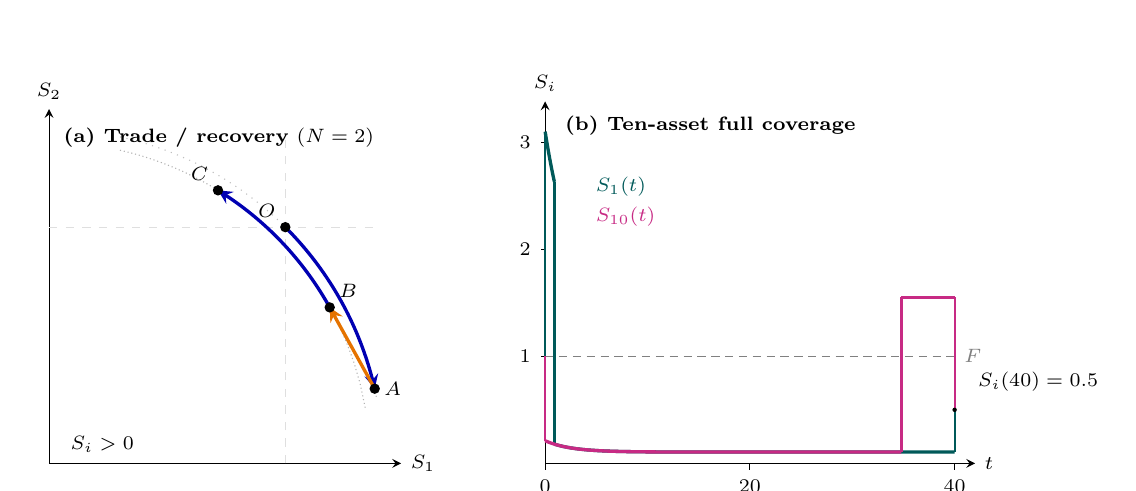
\begin{tikzpicture}[font=\scriptsize,>=stealth]
\pgfmathsetmacro{\sA}{sqrt(1.9)}
\pgfmathsetmacro{\sB}{sqrt(0.1)}
\pgfmathsetmacro{\sC}{1+(\sA-1)*exp(-0.7)}
\pgfmathsetmacro{\sD}{1+(\sB-1)*exp(-0.7)}
\pgfmathsetmacro{\rB}{\sC*\sC+\sD*\sD}
\pgfmathsetmacro{\sE}{sqrt(\sC*\sC-0.9)}
\pgfmathsetmacro{\sF}{sqrt(\sD*\sD+0.9)}
% (a) N=2, F=eta=rho=1: trade h=0.45, recover 0.7, reverse h.
\begin{scope}[x=3.0cm,y=3.0cm]
  \draw[->] (0,0) -- (1.49,0) node[right] {$S_1$};
  \draw[->] (0,0) -- (0,1.5) node[above] {$S_2$};
  \draw[gray!25,dashed] (1,0) -- (1,1.38);
  \draw[gray!25,dashed] (0,1) -- (1.4,1);
  \draw[gray!50,dotted,domain=0.30:1.39,samples=45]
    plot ({\x},{sqrt(2-\x*\x)});
  \draw[gray!60,densely dotted,domain=0.30:1.34,samples=45]
    plot ({\x},{sqrt(\rB-\x*\x)});
  \draw[blue!70!black,very thick,domain=0:0.45,samples=40,->]
    plot ({sqrt(1+2*\x)},{sqrt(1-2*\x)});
  \draw[orange!90!black,very thick,domain=0:0.7,samples=45,->]
    plot ({1+(\sA-1)*exp(-\x)},{1+(\sB-1)*exp(-\x)});
  \draw[blue!70!black,very thick,domain=0:0.45,samples=45,->]
    plot ({sqrt(\sC*\sC-2*\x)},{sqrt(\sD*\sD+2*\x)});
  \fill (1,1) circle (0.022) node[above left] {$O$};
  \fill (\sA,\sB) circle (0.022) node[right] {$A$};
  \fill (\sC,\sD) circle (0.022) node[above right] {$B$};
  \fill (\sE,\sF) circle (0.022) node[above left] {$C$};
  \node[anchor=north west] at (0.02,1.46)
    {\textbf{(a) Trade / recovery} ($N=2$)};
  \node[anchor=west] at (0.05,0.08) {$S_i>0$};
\end{scope}
% (b) N=10, F=eta=1, rho=.4, T=40, full-coverage Appendix D.
% R(t)=H+(sqrt(10)-H) exp(-.4t), directions (a,b,...,b).
\begin{scope}[shift={(6.3cm,0)},x=0.13cm,y=1.36cm]
  \draw[->] (0,0) -- (42,0) node[right] {$t$};
  \draw[->] (0,0) -- (0,3.38) node[above] {$S_i$};
  \draw[densely dashed,gray] (0,1) -- (40,1) node[right] {$F$};
  \foreach \t in {0,20,40}{
    \draw (\t,0) -- (\t,-0.06) node[below] {\t};
  }
  \foreach \p in {1,2,3}{
    \draw (0,\p) -- (-0.45,\p) node[left] {\p};
  }
  \pgfmathsetmacro{\a}{0.9796977322918206}
  \pgfmathsetmacro{\b}{0.0668267688731795}
  \pgfmathsetmacro{\h}{1.5811386521504363}
  \pgfmathsetmacro{\d}{sqrt(10)-\h}
  \draw[teal!70!black,thick] (0,1) -- (0,{sqrt(10)*\a});
  \draw[teal!70!black,very thick,domain=0:0.90218336,samples=12]
    plot (\x,{\a*(\h+\d*exp(-0.4*\x))});
  \draw[teal!70!black,thick]
    (0.90218336,{\a*(\h+\d*exp(-0.4*0.90218336))}) --
    (0.90218336,{\b*(\h+\d*exp(-0.4*0.90218336))});
  \draw[teal!70!black,very thick,domain=0.90218336:40,samples=100]
    plot (\x,{\b*(\h+\d*exp(-0.4*\x))});
  \draw[teal!70!black,thick]
    (40,{\b*(\h+\d*exp(-0.4*40))}) -- (40,0.5);
  \draw[magenta!80!black,thick] (0,1) -- (0,{sqrt(10)*\b});
  \draw[magenta!80!black,very thick,domain=0:34.80222557,samples=100]
    plot (\x,{\b*(\h+\d*exp(-0.4*\x))});
  \draw[magenta!80!black,thick]
    (34.80222557,{\b*(\h+\d*exp(-0.4*34.80222557))}) --
    (34.80222557,{\a*(\h+\d*exp(-0.4*34.80222557))});
  \draw[magenta!80!black,very thick,domain=34.80222557:40,samples=30]
    plot (\x,{\a*(\h+\d*exp(-0.4*\x))});
  \draw[magenta!80!black,thick]
    (40,{\a*(\h+\d*exp(-0.4*40))}) -- (40,0.5);
  \fill (40,0.5) circle (0.8pt) node[anchor=south west,xshift=5pt,yshift=3pt] {$S_i(40)=0.5$};
  \node[anchor=north west] at (1,3.34)
    {\textbf{(b) Ten-asset full coverage}};
  \node[teal!70!black,anchor=west] at (4,2.58) {$S_1(t)$};
  \node[magenta!80!black,anchor=west] at (4,2.30) {$S_{10}(t)$};
\end{scope}
\end{tikzpicture}%
}
\caption{\textbf{Conservation geometry and resilience-driven reachability.}
(a) Under constant impact $g=1$ with $N=2$ and $F=\rho=1$, equal-and-opposite
paired-dollar pulses of magnitude $0.45$ follow the distinct fixed-radius
curves $O\to A$ and $B\to C$; recovery over $T=0.7$ moves the state
from $A$ to $B$ and changes the conserved radius. Both individual executed-dollar
ledgers close, yet $C\ne O$ and the mean log loss is positive.
(b) Selected prices in the analytical ten-asset full-coverage witness with
$\rho=0.4$ and $T=40$; the other eight assets take the same cyclic high
and low roles. Flow-completed pulses produce the jumps. All ten prices
finish at $F/2$ with $X_i(40)=0$. Both panels maintain strictly
positive prices along trajectories evaluated from the model's
analytic primitives.}
\label{fig:conservation-geometry}
\end{figure}


The principal findings are constructive. One ten-asset path makes all prices fall $50\%$ despite exact dollar closure; another sends nine prices arbitrarily close to zero with finite severity-independent turnover and inventory. A third, absolutely continuous path under uniform $\pm25\%$ rolling bands makes five assets close at their lower limits on two consecutive sessions, each losing $43.75\%$. An exclusion bound restricts such repeated lower closes to at most seven assets; the optimum between five and seven remains undetermined. Elasticity barriers, a sharp horizon-dependent full-coverage ceiling, and necessary resource inequalities identify where these results can and cannot occur.

\section{Model and Systemic Drawdown Criterion}\label{sec:micro}\label{sec:model}
We specify a risky-asset reallocation submarket in which every executed sale is matched by an equal-dollar purchase. Settlement and price response are distinct assumptions: the former constrains flows, while the latter determines the induced price motion. All subsequent results use Assumption~\ref{asmp:model} unless stated otherwise.

\begin{assumption}[The resilient paired-dollar market]\label{asmp:model}
Fix $N\ge2$ assets and a finite horizon $[0,T]$. The following jointly define the admissible market.
\begin{enumerate}[label=\textup{(M\arabic*)},leftmargin=2.9em,itemsep=0.20em]
\item \textbf{Positive prices and coordinates.} Each transaction price $S_i(t)$ is strictly positive and initially $S_i(0)=F>0$. A strictly increasing $C^1$ coordinate $q_i=\phi_i(S_i)$ preserves price priority. The analysis concerns deterministic admissible execution paths.
\item \textbf{Trade and execution accounting.} Executed share change is the signed quantity $\dd\theta_i$; unsigned volume counts its absolute increments, not both counterparties twice. Executions obey marginal-price settlement $\dd X_i=S_i\dd\theta_i$. Matching uses price priority conditional on an order book; the effective price response is a separately imposed, positive, locally $C^2$ function $g(S)$, such that $\dd S_i|_{\rm trade}=g(S_i)\dd\theta_i$.
\item \textbf{No fundamental news and resilience.} The benchmark $F$ stays fixed. Between trades, prices recover toward $F$ at a common constant rate $\rho>0$: $\dot S_i=-\rho(S_i-F)$ in the absence of execution. The response function $g$ and $\rho$ are specified exogenously.
\item \textbf{Paired-dollar transaction network.} Each permitted transaction moves an equal executed-dollar amount between a source asset and a destination asset: $\dd\bm X=B\dd\bm z$, where $B$ is the oriented incidence matrix of the complete bidirectional graph, $\dd\bm z\ge0$, and $\one^\top B=0$. This condition specifies an idealized paired-reallocation submarket without external cash inflows.
\item \textbf{Admissible controls and terminal closure.} Paths are piecewise continuous and of finite execution variation, with finitely many marginally settled instantaneous pulses allowed; every price remains positive and required sale inventory is available without short sales. The terminal comparison imposes $X_i(T)=0$ for \emph{each} asset, not $\theta_i(T)=\theta_i(0)$. Where resource caps are claimed, identical total paired-dollar turnover and per-asset starting share limits are imposed across markets.
\end{enumerate}
\end{assumption}



\paragraph{Price-level resilience as a modeling choice}
Assumption (M3) fixes recovery in the \emph{price} coordinate,
$\dot S=-\rho(S-F)$, separately from the effective trade response in (M2).
Order-book volume recovery is a different model except at constant impact~\citep{RochSoner2013}. The structural elasticity barriers below are proved specifically under price-level recovery (M3).

\paragraph{Two levels of executed-dollar accounting}
Condition (M4) matches dollars within each transfer, while
(M5) closes each asset's cumulative signed-dollar ledger
at $T$; the associated inventory accounting follows from~\eqref{eq:cost}.

\paragraph{Finite-variation paths and marginally settled pulses}
For absolutely continuous controls the differential notation is classical. At a jump, settlement follows the within-event price path rather than valuing the entire transaction at an endpoint. Hold physical time fixed and parameterize a directed edge $e:i\to j$ carrying dollar mass $z>0$ by $a\in[0,z]$:
\begin{equation}\label{eq:pulse-flow}
\frac{\dd \widetilde S_i}{\dd a}=-\frac{g(\widetilde S_i)}{\widetilde S_i},\quad
\frac{\dd \widetilde S_j}{\dd a}=\frac{g(\widetilde S_j)}{\widetilde S_j},\quad
\frac{\dd\widetilde\theta_i}{\dd a}=-\frac{1}{\widetilde S_i},\quad
\frac{\dd\widetilde\theta_j}{\dd a}=\frac{1}{\widetilde S_j}.
\end{equation}
The resulting endpoint flows satisfy $\Delta X_i=-z$, $\Delta X_j=z$ and $\Delta\Phi(S_i)=-z$, $\Delta\Phi(S_j)=z$. Equivalently, a single-share impulse is evaluated by solving $\dd\widetilde S/\dd\xi=g(\widetilde S)$ and integrating $\int\widetilde S\,\dd\xi$ along that response trajectory. These \emph{flow-completed} (Marcus-type) updates preserve the ordinary chain rule; graph-completed solutions of bounded-variation impulsive control systems provide a related analytic framework \citep{BressanRampazzo1988}. Finite pulses on distinct edges are processed in their prescribed order. A pulse is admissible only while all intermediate prices remain strictly positive. These rules specify the interpretation of all jump expressions in what follows.

\paragraph{From the conditional matching map to an effective response} Fix a frozen book $\mathcal B$ with locally positive continuous share-depth density $\rho_S(S;\mathcal B)$. A one-sided sweep whose signed marginal share size is $\dd\theta$ obeys the local relation
\begin{equation}\label{eq:frozen-depth}
\dd\theta=\rho_S(S;\mathcal B)\dd S,
\qquad \rho_q(q;\mathcal B)\dd q=\rho_S(S;\mathcal B)\dd S.
\end{equation}
The exact discrete version uses the generalized inverse of the book's cumulative depth. In the continuous approximation, changing $q=\phi(S)$ changes the density numerically through the Jacobian, not the matching priority. The relation concerns the marginal executed price; dynamic midpoint evolution, replenishment, and cross-impact require additional dynamics. In large-trader and supply-curve models, execution prices likewise respond to trading activity \citep{BankBaum2004,CetinJarrowProtter2004}. Assumption (M2) uses the frozen-book relation to motivate the effective state-dependent response $g(S)=1/\rho_S^{\rm eff}(S)$.

\paragraph{Price dynamics for $N$ assets} Under the full market specification, the level-price law is
\begin{equation}\label{eq:level-dynamics}
\dd S_i(t)=-\rho\big(S_i(t)-F\big)\dd t+g(S_i(t))\dd\theta_i(t),\qquad \dd X_i=S_i\dd\theta_i.
\end{equation}
Choose the strictly monotone generalized coordinate $q_i=\log(S_i/F)$. Conversion to paired dollars gives
\begin{equation}\label{eq:log-impact}
\dd q_i\big|_{\rm trade}=\frac{g(S_i)}{S_i^2}\dd X_i.
\end{equation}
Combining this conversion, transaction pairing, and resilience yields the full multiasset system
\begin{equation}\label{eq:master}
\dd\bm q=-\rho(\one-e^{-\bm q})\dd t+D(\bm q)B\dd\bm z,\qquad
D_{ii}(\bm q)=\frac{g(Fe^{q_i})}{F^2e^{2q_i}}.
\end{equation}
The exponential acts componentwise. This log coordinate is convenient for measuring losses, but executed dollars admit a simpler \emph{response-adapted} coordinate. Let $y_i=\Phi(S_i)$ with $\Phi$ as in~\eqref{eq:phi-intro}. It is strictly increasing and satisfies $\Phi(F)=0$. Moreover, among differentiable coordinates $\psi$ normalized by $\psi(F)=0$, the requirement that each marginal trade obey $\dd\psi(S)|_{\rm trade}=\dd X$ forces $\psi'(S)g(S)=S$ and thus uniquely selects $\psi=\Phi$. Define the restoring response
\[
\mathcal R(y)=\frac{S(S-F)}{g(S)},\qquad S=\Phi^{-1}(y).
\]
The entire multiasset market then has the \emph{trade-normalized form}
\begin{equation}\label{eq:normal-form}
\dd\bm y=B\dd\bm z-\rho\mathcal R(\bm y)\dd t,\qquad\one^\top B=0,
\end{equation}
where $\mathcal R$ acts componentwise and the execution rule applies also to flow-completed pulses. Trading is therefore an additive zero-sum input; all nonlinear price-state dependence has moved into the restoring term and the inverse map $S=\Phi^{-1}(y)$. The transformed state space is $\mathcal J^N$, where $\mathcal J=\Phi((0,\infty))$. For $g_p(S)=\eta(S/F)^p$, the range is $(-F^2/[\eta(2-p)],\infty)$ for $p<2$, $\mathbb R$ for $p=2$, and $(-\infty,F^2/[\eta(p-2)])$ for $p>2$. Thus additive trading inputs do not remove strict price positivity or execution constraints. This change of coordinates does not alter which price states are reachable. With $\rho=0$ the traded sum of generalized coordinates is exactly conserved.

Geometrically, trading moves the state along level sets of
$H=\sum_i\Phi(S_i)$, while recovery moves it across them.

\begin{definition}[Terminal systemic drawdown]\label{def:crash}
Let $L_i(T)=\log[F/S_i(T)]$ and $\overline L(T)=N^{-1}\sum_i L_i(T)$. The $k$th-largest loss, where $k=\lceil\alpha N\rceil$, is $Q_\alpha(T)$. Define
\begin{equation}\label{eq:crash}
\Cris_\alpha(T)=\min\{\overline L(T),Q_\alpha(T)\}.
\end{equation}
For $\delta>0$, a \emph{terminal crisis} occurs when $\Cris_\alpha(T)\ge\delta$. Thus the mean loss and at least $k$ individual losses must each reach $\delta$. The target is selected independently of the price-response function.
\end{definition}

The mean-loss component measures the decline of the equally weighted geometric price index, since
\[
\overline L(T)=-\log\!\left[\left(\prod_{i=1}^{N}\frac{S_i(T)}{F}\right)^{1/N}\right].
\]
The criterion therefore combines geometric-index deterioration with a breadth requirement. Arithmetic price averages and market-capitalization-weighted indices are different aggregates; for example, the $p=1$ market below can have $\Cris_\alpha(T)>0$ while $\sum_i S_i(T)=NF$.

The discrete coverage rule is material: for $N=3$, $\alpha=0.9$ means $k=3$, so it requires a fall in all three assets. More generally, the contrast $k=N$ versus $k<N$ determines whether a compensating asset exists at all. This same distinction appears first in the A/B/C classification and later in the multiday cross-asset capacity inequality. A first-passage event $\tau_{\alpha,\delta}=\inf\{t:\Cris_\alpha(t)\ge\delta\}$ is different from a \emph{terminal} crisis under dollar closure; we study the latter.

\begin{definition}[Turnover, share inventory and terminal critical budget]\label{def:budget}
For an admissible path $\gamma$, set
\begin{equation}\label{eq:resource}
M(\gamma)=\sum_e\int_0^T\dd z_e,\qquad
H_i^-(\gamma)=\int_0^T\big(-\dd\theta_i\big)_+.
\end{equation}
Under allowed initial inventory $H_i$ and terminal dollar closure, define
\begin{equation}\label{eq:minbudget}
M_*^{\rm end}=\inf\{M(\gamma): X_i(T)=0\ \forall i,\ \Cris_\alpha(T)\ge\delta,\ \gamma\text{ admissible}\},
\end{equation}
with $\inf\varnothing=+\infty$. A paired dollar transfer is counted once in $M$, although it appears with opposite signs in two asset ledgers.
\end{definition}

\paragraph{Execution-cost identity} Define
\begin{equation}\label{eq:E}
E(S)=\int_F^S\frac{u-F}{g(u)}\dd u\ge0.
\end{equation}
For any admissible path beginning at $F$ the execution-cost identity is
\begin{equation}\label{eq:cost}
\int_0^T S_i\dd\theta_i=F[\theta_i(T)-\theta_i(0)]+E(S_i(T))
+\rho\int_0^T\frac{(S_i-F)^2}{g(S_i)}\dd t.
\end{equation}
Thus a \emph{share-flat} round trip has nonnegative executed cost under (M2)--(M3). Appendix~\ref{app:accounting} proves the accounting identity and its consequences for admissible controls.

\paragraph{Comparison with share-flat trading}
For example, with $g\equiv\eta$, a single asset purchased by a sufficiently small $a>0$ shares at time $0$ and sold by $a$ shares at time $T$ has $\theta(T)=\theta(0)$ but terminal price $S(T)=F-\eta a(1-e^{-\rho T})<F$; its net executed dollars are not zero and the positive cost in \eqref{eq:cost} is paid through the cash account. Conversely, under (M4), requiring every asset to be share-flat \emph{as well as} terminally dollar-flat would force $\sum_i[E(S_i(T))+\rho\int_0^T(S_i-F)^2/g(S_i)\,\dd t]=0$. Thus there can be no positive-time dissipative price excursion under both closures together.

\section{Structural Barriers and Robustness}\label{sec:barriers}
The normal form~\eqref{eq:normal-form} supplies a conserved scalar during trading. Write $H(\bm S)=\one^\top\bm y=\sum_i\Phi(S_i)$. Summing over assets cancels every matched dollar transfer and leaves only recovery:
\begin{equation}\label{eq:potential-law}
\dd H=-\rho\sum_{i=1}^N\mathcal R(y_i)\dd t
=-\rho\sum_{i=1}^N\frac{S_i(S_i-F)}{g(S_i)}\dd t.
\end{equation}
The sign of the restoring drift depends on the price configuration.
Structural exclusion therefore requires curvature conditions on the
response-adapted coordinate. Introduce the elasticity
\begin{equation}\label{eq:elasticity}
e(S)=\frac{Sg'(S)}{g(S)}.
\end{equation}
The derivatives of $\Phi$ and $G(x)=\Phi(Fe^x)$ are
\begin{equation}\label{eq:curvature}
\Phi''(S)=\frac{1-e(S)}{g(S)},\qquad
G''(x)=\frac{S^2}{g(S)}\,[2-e(S)],\quad S=Fe^x.
\end{equation}
The distinction between these two curvatures tracks the definition of systemic loss. A barrier to \emph{every asset} being below its benchmark is weaker than a barrier to our functional, which also involves the \emph{average} log loss. Thus the same coordinate can produce two different exclusion statements.


\begin{theorem}[Barrier to a decline of every asset]\label{thm:barrier1}
If $e(S)\ge1$ at all prices attainable by admissible paths, then $S_i(t)<F$ for every $i$ is impossible at any time $t$. In particular, no positive crisis with $k=N$ is reachable.
\end{theorem}
\begin{proof}
Equation~\eqref{eq:curvature} makes $\Phi$ concave. Its tangent inequality at $S$ is $\Phi(F)\le\Phi(S)+\Phi'(S)(F-S)$, hence $(S-F)\Phi'(S)\le\Phi(S)$. Consequently \eqref{eq:potential-law} implies $\dot H\ge-\rho H$ between trades; pulses preserve $H$. Since $H(0)=0$, comparison gives $H(t)\ge0$. If every $S_i(t)<F$, strict monotonicity and $\Phi(F)=0$ instead imply $H(t)<0$, a contradiction.
\end{proof}

\begin{theorem}[Barrier to a systemic crisis of any breadth]\label{thm:barrier2}
If $e(S)\ge2$ on the admissible price range, then for every admissible control, $N\ge2$, $\alpha\in(0,1]$ and $t\in[0,T]$,
\begin{equation}\label{eq:no-crash}
\Cris_\alpha(t)\le0.
\end{equation}
Thus no strictly positive systemic terminal-crisis threshold can be reached.
\end{theorem}
\begin{proof}
The preceding theorem gives $H(t)\ge0$. The second identity in \eqref{eq:curvature} makes $G(x)=\Phi(Fe^x)$ concave and strictly increasing. Jensen's inequality yields
\[
0\le\frac{H(t)}N=\frac1N\sum_iG(q_i(t))
\le G\!\left(\frac1N\sum_iq_i(t)\right).
\]
As $G(0)=0$ and $G$ is strictly increasing, $\sum_iq_i(t)\ge0$. Hence the mean loss $\overline L(t)=-N^{-1}\sum_iq_i(t)$ is nonpositive; Definition~\ref{def:crash} implies \eqref{eq:no-crash}.
\end{proof}

The barriers hold for the entire admissible path without requiring terminal dollar closure. When the elasticity bound holds only near $F$, the argument applies while prices stay in that region; execution resources and network constraints may impose further restrictions. Section~\ref{sec:regimes} compares how the attainable set changes across response functions.

\subsection{Robustness to unmatched dollar flow and impact heterogeneity}
\label{subsec:barrier-robustness}
The exclusion in Theorem~\ref{thm:barrier2} uses both a common
price-response function and exact dollar pairing. The local logarithmic
price response per executed dollar is
$\lambda(S)=g(S)/S^2$, with elasticity
\[
\frac{\dd\log\lambda(S)}{\dd\log S}=e(S)-2.
\]
Thus the threshold $e\ge2$ states that this model's local
per-dollar log-impact does not increase as the price falls.
We quantify two departures from the hypotheses of the exclusion theorem
while retaining fixed fundamentals and common price-level recovery.

\begin{proposition}[Stability under unmatched dollar flow]
\label{prop:unbalanced-stability}
Suppose $S_i(0)=F$, all prices remain positive, and the homogeneous
response $g>0$ and common recovery rate $\rho>0$ satisfy
$e(S)\ge2$ on an interval containing $F$ and every attained price.
For absolutely continuous executed-dollar flows, relax exact pairing
to $\sum_i\dot X_i(t)=\varepsilon(t)$ with
$\varepsilon\in L^1([0,T])$. Then, for all $t\in[0,T]$ and
$\alpha\in(0,1]$,
\[
\begin{aligned}
\Cris_\alpha(t)\le\overline L(t)
&\le-\frac{g(F)}{NF^2}
 \int_0^t e^{-\rho(t-s)}\varepsilon(s)\,\dd s\\
&\le\frac{g(F)}{NF^2}
 \int_0^t e^{-\rho(t-s)}[-\varepsilon(s)]_+\,\dd s.
\end{aligned}
\]
\end{proposition}
\begin{proof}
Let $H(t)=\sum_i\Phi(S_i(t))$, where $\Phi(F)=0$
and $\Phi'(S)=S/g(S)$. Concavity of $\Phi$, implied by
$e\ge2$, gives $(S-F)\Phi'(S)\le\Phi(S)$. Hence
\[
\dot H=\varepsilon-\rho\sum_i(S_i-F)\Phi'(S_i)
\ge\varepsilon-\rho H,
\]
and $H(0)=0$ implies
$H(t)\ge\int_0^t e^{-\rho(t-s)}\varepsilon(s)\,\dd s$.
Moreover, $G(q)=\Phi(Fe^q)$ is concave and
$G'(0)=F^2/g(F)$, so its tangent inequality yields
\[
H(t)=\sum_iG(q_i(t))
\le\frac{F^2}{g(F)}\sum_iq_i(t)
=-\frac{NF^2}{g(F)}\overline L(t).
\]
Combining these bounds and discarding the nonnegative part of
$\varepsilon$ in the weighted integral proves the claim.
\end{proof}

Here $\varepsilon$ measures the unmatched executed-dollar rate
\emph{within the selected asset set}; it need not represent a net
cash flow into the wider market. Exact pairing recovers
Theorem~\ref{thm:barrier2}. The estimate does not require
terminal dollar-ledger closure.

\begin{proposition}[Weighted-flow bound for heterogeneous quadratic impact]
\label{prop:heterogeneous-quadratic}
Suppose $S_i(0)=F$ and
$g_i(S)=\eta_i(S/F)^2$, where $\eta_i>0$, with common
$F>0$ and $\rho>0$. For positive absolutely continuous
trajectories set $\kappa_i=\eta_i/F^2$ and
$\omega(t)=\sum_i\kappa_i\dot X_i(t)$.
Then, for all $t\in[0,T]$ and $\alpha\in(0,1]$,
\[
\begin{aligned}
\Cris_\alpha(t)\le\overline L(t)
&\le-\frac1N\int_0^t e^{-\rho(t-s)}\omega(s)\,\dd s\\
&\le\frac1N\int_0^t e^{-\rho(t-s)}[-\omega(s)]_+\,\dd s.
\end{aligned}
\]
Writing $\bar\kappa=N^{-1}\sum_i\kappa_i$ and
$\varepsilon=\sum_i\dot X_i$, the weighted imbalance decomposes as
\[
\omega=\bar\kappa\,\varepsilon+
\sum_i(\kappa_i-\bar\kappa)\dot X_i.
\]
Consequently exact dollar pairing alone need not eliminate the
weighted flow when the impact strengths differ.
\end{proposition}
\begin{proof}
With $q_i=\log(S_i/F)$, the impact law becomes
$\dot q_i=-\rho(1-e^{-q_i})+\kappa_i\dot X_i$.
Jensen's inequality and $e^x\ge1+x$ imply
\[
\begin{aligned}
\frac{\dd}{\dd t}\overline L(t)
&=\rho\left(1-\frac1N\sum_i e^{-q_i}\right)
-\frac{\omega}{N}\\
&\le\rho(1-e^{\overline L})-\frac{\omega}{N}
\le-\rho\overline L-\frac{\omega}{N}.
\end{aligned}
\]
The result follows by comparison from $\overline L(0)=0$.
\end{proof}

\paragraph{A terminally dollar-closed counterexample}
The loss of the homogeneous barrier is possible even with
exact dollar pairing \emph{and} terminal closure. Take $N=2$,
$\kappa_1>\kappa_2>0$, and two matched executed-dollar pulses:
$(\dd X_1,\dd X_2)=(a,-a)$ at time $0$, followed by
$(-a,a)$ at time $T>0$. Both asset ledgers close exactly,
and total paired-dollar turnover is $2a$.
Writing $r=e^{-\rho T}\in(0,1)$, the terminal log prices are
\[
\begin{aligned}
q_1(T)&=\log\bigl(1+r(e^{\kappa_1a}-1)\bigr)-\kappa_1a,\\
q_2(T)&=\log\bigl(1+r(e^{-\kappa_2a}-1)\bigr)+\kappa_2a.
\end{aligned}
\]
For sufficiently small $a>0$, Taylor expansion gives
\[
\overline L(T)=
\frac{(1-r)(\kappa_1-\kappa_2)}2\,a+O(a^2)>0,
\qquad
Q_{1/2}(T)=(1-r)\kappa_1a+O(a^2)>0.
\]
Therefore $\Cris_{1/2}(T)>0$, although each response has
elasticity $e_i=2$. Prices remain strictly positive, and a
sufficient initial share inventory covers the finite sales.
This construction uses instantaneous pulses and does not impose a
gross-rate cap. The common-impact hypothesis of Theorem~\ref{thm:barrier2}
fails in this example.

The two perturbation estimates isolate departures from matching
and homogeneous impact strength. They keep $F$ and $\rho$ fixed;
time-varying fundamentals, heterogeneous restoration, and
nonseparable cross-impact require separate analysis.

\section{Reachability Regimes under Power-Law Impact}\label{sec:regimes}
To compare exclusion and reachability under matched assumptions, we vary only the response shape in the family
\begin{equation}\label{eq:power}
 g_p(S)=\eta\left(\frac SF\right)^p,\qquad p\in\{2,1,0\},\quad \eta>0.
\end{equation}
All three markets have identical $N,T,F,\rho,\eta$, identical initial prices and initial \emph{impact}, the same paired-dollar trading network, and, when compared numerically, the same turnover and inventory caps. They differ only in the exponent $p$. In the log-dollar equation \eqref{eq:master},
\begin{equation}\label{eq:powerd}
 D_{ii}^{(p)}(q_i)=\frac\eta{F^2}e^{(p-2)q_i},\qquad e(S)=p.
\end{equation}
The same coordinate formula integrates explicitly for every exponent:
\[
\Phi_p(S)=\begin{cases}
\displaystyle \frac{F^p}{\eta(2-p)}\big(S^{2-p}-F^{2-p}\big),&p\ne2,\\[4pt]
\displaystyle \frac{F^2}{\eta}\log(S/F),&p=2.
\end{cases}
\]
Consequently, paired trades conserve a quantity proportional to $\sum_iS_i^2$, $\sum_iS_i$, or $\sum_i\log S_i$ for $p=0,1,2$, respectively. Recovery evolves these quantities between trades. Figure~\ref{fig:response} shows the corresponding instantaneous response per executed dollar: below $F$, the $p=0$ response amplifies dollar trades most strongly.

\Needspace{8\baselineskip}
\begin{theorem}[A/B/C reachability regimes]\label{thm:ABC}
Let $N\ge2$ and $k=\lceil\alpha N\rceil<N$. Compare the three markets in \eqref{eq:power} under the same model protocol.
\begin{enumerate}[label=\textup{(\Alph*)},leftmargin=2em,itemsep=0.15em]
\item \textbf{Barrier market ($p=2$):} $\Cris_\alpha(t)\le0$ for every admissible path and every horizon.
\item \textbf{Inventory-bounded market ($p=1$):} positive but sufficiently small terminal systemic drawdowns are reachable. If every asset starts with a fixed finite inventory cap $H_0$ and short selling is forbidden, the terminal crisis severity is bounded above independently of the trade sequence.
\item \textbf{Market with unbounded partial-coverage losses ($p=0$):} for every fixed $N\ge2$ and $k<N$, there exists a sufficiently long but finite horizon $T$ and finite constants $M_0,H_0$ such that, for \emph{every} finite $\delta>0$, an admissible positive-price path with $M\le M_0$, $H_i^-\le H_0$, and $X_i(T)=0$ attains $\Cris_\alpha(T)>\delta$.
\end{enumerate}
The constants in (C) may depend on $N,T,F,\rho,\eta$, but not on $\delta$. They do not remain uniform as $N\to\infty$.
\end{theorem}
\begin{proof}
(A) is Theorem~\ref{thm:barrier2}; (B) follows from Proposition~\ref{prop:two-pulse} and the inventory inequality~\eqref{eq:inventoryb}. We give the constructive mechanism for (C), with the auxiliary estimates in Appendix~\ref{app:severe}. Put $m=N-1$ and take $g\equiv\eta$. Paired-dollar pulses preserve $R^2=\sum_iS_i^2$. Choose a fixed small $c>0$, a compensator direction $b\in(0,1/5)$, and $a=\sqrt{1-b^2-(m-1)c^2}>b,c$. During stage $j$, set
\[
\begin{aligned}
 \bm u_j&=(c,\ldots,\underbrace{a}_{j},\ldots,c,b),
 &H_b&=a+(m-1)c+b,\\
 \bm S(t)&=R_b(t)\bm u_j,
 &R_b(t)&=F\bigl[H_b+(\sqrt N-H_b)e^{-\rho t}\bigr].
\end{aligned}
\]
The necessary continuous rates are
$\dot\theta_i=(\rho F/\eta)(u_{j,i}H_b-1)$, whose executed-dollar sum vanishes since $\sum_i u_{j,i}^2=1$ and $\sum_i u_{j,i}=H_b$. Switching directions by strictly positive squared-price interpolation yields paired fixed-radius pulses. A final pulse sets the first $m$ terminal prices to $\varepsilon>0$ and the compensator to $\sqrt{R_b(T)^2-m\varepsilon^2}$.

The exact dollar-ledger identity~\eqref{eq:Xledger} gives opposite signs for the compensator's terminal balance at $b=0$ and $b=1/5$ for fixed sufficiently long finite $T$ and sufficiently small $\varepsilon$. By continuity an interior $b(\varepsilon)$ closes this ledger. The strictly positive recovery-weight difference
$W(t)=(a-c)R_b(t)[(a+c)R_b(t)-F]$
permits partitioning the horizon into $m$ equal $W$-integral intervals. Each target takes the high role on exactly one interval, making the target ledgers equal. As paired trading makes their total balance zero after the compensator closes, each individual target ledger must also vanish.

The pulses remain positive and finite in number and the radial scale stays bounded. In particular, Appendix~\ref{app:severe} proves
\[
 M\le\frac{N^3F^2}{4\eta}+\frac{\rho NF^2T}{\eta},\qquad
 H_i^-\le\frac{NF\sqrt N+\rho FT(\sqrt N+1)}{\eta},
\]
independent of $\varepsilon$. Hence both the mean log loss and the $k$th-largest log loss diverge as $\varepsilon\downarrow0$ for $k<N$, proving (C).
\end{proof}

\begin{figure}[H]
\centering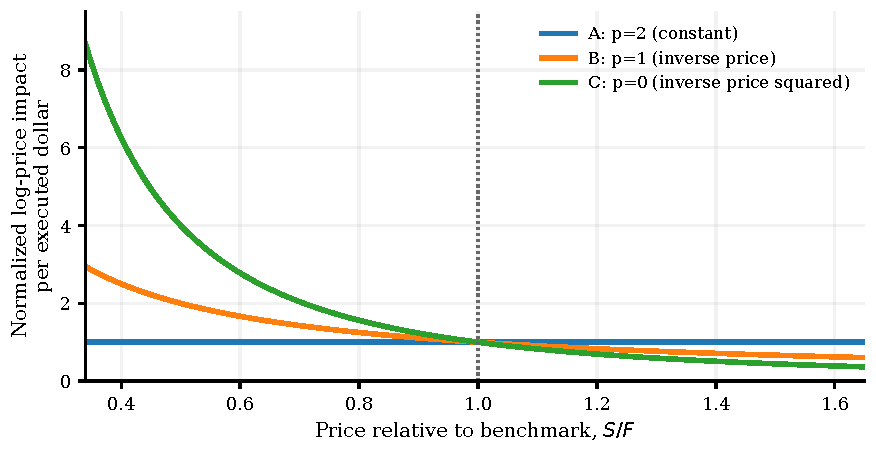
\includegraphics[width=0.82\linewidth]{figures/response_regimes.pdf}
\caption{\textbf{A single response family, three price sensitivities.} The plot shows the model-implied instantaneous \emph{log-price change per executed dollar}, normalized by its common initial value. All curves coincide at $S=F$.}\label{fig:response}
\end{figure}

The condition $k<N$ in (C) is essential: at least one asset must be available to carry the compensating flow. Finite gross share rates further constrain the compensating asset's \emph{capacity}.

For $p=1$, the inventory potential from \eqref{eq:E} is
\begin{equation}\label{eq:inventoryb}
E_1(Fe^{-L})=\frac{F^2}{\eta}\left(L+e^{-L}-1\right).
\end{equation}
By \eqref{eq:cost}, terminal dollar closure and no short selling imply $E_1(S_i(T))\le FH_0$. Since $L+e^{-L}-1\to\infty$ as $L\to\infty$, no fixed finite inventory can support arbitrarily severe losses of the requisite $k$ assets. By contrast, for $p=0$, $E_0(S)=(S-F)^2/(2\eta)$ remains bounded as $S\downarrow0$; this makes the construction in (C) possible but does not by itself prove reachability.

\begin{proposition}[Local all-asset decline]\label{prop:three-pulse}
If $g$ is $C^3$ near $F$ and $e(F)<1$, then for every $N\ge2$ there exists a terminally dollar-closed, positive-price, small-amplitude three-pulse control under which \emph{every} $S_i(T)<F$. With $c=g(F)/F^2$ and $r=e^{-\rho T/2}$, the losses of a zero-sum impulse direction $\bm u$ with every $u_i\ne0$ satisfy
\begin{equation}\label{eq:three-pulse}
L_i(T)=\frac{1-e(F)}2c^2h^2u_i^2r(1-r^2)+O(h^3)>0
\end{equation}
for sufficiently small $h>0$.
\end{proposition}
\begin{proof}
Apply the executed-dollar pulses $h\bm u$, $-(1+r)h\bm u$, $rh\bm u$ at $0,T/2,T$. They are pairwise dollar-balanced and sum to zero for every asset. Taylor expansion in the coordinate $y=\Phi(S)$ gives \eqref{eq:three-pulse}; details appear in Appendix~\ref{app:local}.
\end{proof}

\begin{proposition}[Local partial-coverage decline]\label{prop:two-pulse}
Let $k<N$, $e_0=e(F)<2$, $c=g(F)/F^2$, and $r=e^{-\rho T}<2-e_0$. Select a zero-sum dollar direction with at least $k$ positive components and execute $h\bm u$ at time $0$ and $-h\bm u$ at time $T$. Then $\Cris_\alpha(T)>0$ for all sufficiently small $h>0$, and
\begin{equation}\label{eq:two-pulse}
\overline L(T)=\frac{c^2h^2}{2N}(1-r)(2-e_0-r)\sum_iu_i^2+O(h^3).
\end{equation}
\end{proposition}
\begin{proof}
The individual losses satisfy $L_i(T)=c(1-r)hu_i+O(h^2)$, while the first-order term vanishes when averaged because $\sum_i u_i=0$. The strictly positive quadratic coefficient in \eqref{eq:two-pulse} proves the result. See Appendix~\ref{app:local}.
\end{proof}

The divergence in the third response regime is a finite-resource, strictly positive-price existence result; its construction and uniform bounds, rather than a separate numerical parameter sweep, provide the evidence.

\paragraph{The continuous power-law spectrum}
The local response elasticity here differs from cumulative metaorder-impact scaling~\citep{BucciEtAl2019,KyleObizhaeva2023}. The three canonical markets in Theorem~\ref{thm:ABC} are part of a
continuous family: retain the expression for $g_p$ in
\eqref{eq:power}, now allowing $0\le p\le2$. Since $e(S)=p$,
the elasticity barriers and the local constructions distinguish
two critical exponents. In geometric terms,
$\Phi_p''(S)=(1-p)/g_p(S)$, while
$G_p''(q)=F^2(2-p)e^{(2-p)q}/\eta$ for
$G_p(q)=\Phi_p(Fe^q)$: the two curvatures reach their
respective thresholds at $p=1$ and $p=2$.
For $0\le p<2$, the dollar-coordinate
distance to zero is finite, whereas the share-coordinate distance
changes character at $p=1$:
\[
-\Phi_p(0^+)=\frac{F^2}{\eta(2-p)},\qquad
-\Psi_p(0^+)=
\begin{cases}
\displaystyle\frac{F}{\eta(1-p)},&0\le p<1,\\[3pt]
+\infty,&1\le p<2.
\end{cases}
\]
The inventory potential in~\eqref{eq:E}, evaluated at
$S=Fe^{-L}$, is for $p\ne1,2$
\[
E_p(Fe^{-L})=\frac{F^2}{\eta}
\left[\frac{e^{(p-1)L}-1}{p-1}
-\frac{1-e^{-(2-p)L}}{2-p}\right].
\]
For $0\le p<1$, its zero-price limit is
$E_p(0^+)=F^2/[\eta(1-p)(2-p)]<\infty$.
Proposition~\ref{prop:three-pulse} also makes a small, simultaneous
decline of every asset locally reachable in this regime.
Finiteness of the coordinate distances and inventory potential
alone does not establish global reachability. Theorem~\ref{thm:sublinear-severe}
below supplies the required constructive extension of uniform-budget
severe partial-coverage losses to every fixed $0\le p<1$.

At $p=1$, Theorem~\ref{thm:barrier1} excludes simultaneous declines,
while Proposition~\ref{prop:two-pulse} gives local partial-coverage
losses at every positive horizon. The potential~\eqref{eq:inventoryb}
then grows linearly with $L$. For $1<p<2$, simultaneous declines
remain excluded, but local partial-coverage losses are reachable
under the sufficient horizon condition
$e^{-\rho T}<2-p$, or $T>-\log(2-p)/\rho$.
Here the dollar distance is still finite while
$E_p(Fe^{-L})\sim F^2e^{(p-1)L}/[\eta(p-1)]$ as $L\to\infty$.
Indeed, if terminal executed-dollar flows vanish, short sales
are prohibited, and the initial inventory of a qualifying asset
is at most $H_0$,~\eqref{eq:share-bound} implies
\[
L\le\frac{1}{p-1}\log\!\left[
1+(p-1)\left(\frac{\eta H_0}{F}+\frac{1}{2-p}\right)
\right],\qquad 1<p<2.
\]
Thus, for fixed $p\in(1,2)$, the inventory-based severity
ceiling scales at most logarithmically in large $H_0$, rather than
linearly as for $p=1$. At the second threshold $p=2$,
$-\Phi_2(0^+)$ diverges and Theorem~\ref{thm:barrier2}
excludes every positive systemic crisis measure. These thresholds distinguish local and global reachability as well
as the boundary resource singularities.


\Needspace{14\baselineskip}
\begin{theorem}[Uniform-resource severe partial-coverage losses for sublinear impact]\label{thm:sublinear-severe}
Fix $N\ge2$, $k=\lceil\alpha N\rceil<N$, positive $F,\eta,\rho$,
and an exponent $0\le p<1$ in
$g_p(S)=\eta(S/F)^p$. There exist a finite horizon $T>0$
and finite constants $M_0,H_0$, depending on these fixed
market parameters but not on the loss threshold, such that for
every $\delta>0$ an admissible positive-price,
terminally dollar-closed path, using finitely many
flow-completed pulses and absolutely continuous controls
between them, satisfies
\[
\Cris_\alpha(T)>\delta,\qquad
M(\gamma)\le M_0,\qquad
H_i^-(\gamma)\le H_0\quad(1\le i\le N).
\]
No constants uniform as $p\uparrow1$ and no prescribed
finite gross execution-rate cap are asserted.
\end{theorem}
\begin{proof}
Put $\nu=2-p>1$. Paired-dollar pulses preserve
$\sum_iS_i^\nu$, so their positive-price orbits are
$\ell^\nu$ spheres. The $\ell^\nu$-radial construction in
Appendix~\ref{app:sublinear-severe} first closes the
compensating asset's dollar ledger using a direction
parameter $b_\varepsilon\in(b_-,\bar b)$, where the
positive lower bound $b_->0$ and the finite horizon
are independent of $\varepsilon$. A partition by equal
positive recovery-weight integrals then closes every
target asset's ledger. On continuous control stages,
all direction coordinates are at least
$d_*=\min\{c,b_-\}>0$, which bounds their share rates.
On each of the finitely many transaction pulses,
the gross share variation remains finite uniformly
as $\varepsilon\downarrow0$, because
\[
\frac{F^p}{\eta}\int_0^{FN^{1/\nu}}u^{-p}\dd u
=\frac{F}{\eta(1-p)}\,N^{(1-p)/\nu}<\infty.
\]
The $\ell^\nu$ radius also bounds pulse-dollar variation;
the appendix combines these estimates with bounded
continuous turnover to give constants $M_0,H_0$
independent of $\varepsilon$ and hence of $\delta$.
\end{proof}

\subsection{A sharp boundary when every asset must fall}\label{sec:allcoverage}
Market C relies on $k<N$. To see why the breadth condition matters beyond a technical assumption, keep \emph{the same constant-impact response} but change the target to $k=N$. There is then no nonqualifying asset available to compensate the other $N-1$ terminal losses. In the sharp construction, the high-price role rotates among assets during recovery; finite recovery time limits how far their common terminal price can fall. The model therefore yields an exact horizon-dependent ceiling, even before a fixed execution budget is imposed.

\begin{theorem}[Sharp all-asset horizon threshold]\label{thm:critical}
Under Assumption~\ref{asmp:model} with $g(S)=\eta$ and $k=N$, define
\begin{equation}\label{eq:critical}
\delta_{\mathrm{crit}}(N,T)=
\log\frac{\sqrt N}{1+(\sqrt N-1)e^{-\rho T}}.
\end{equation}
For every $\delta\in(0,\delta_{\mathrm{crit}}(N,T))$, some admissible terminally dollar-closed control reaches $\Cris_1(T)\ge\delta$ with finite turnover and sufficiently large finite inventory. If $\delta\ge\delta_{\mathrm{crit}}(N,T)$, no such positive-price path exists. Thus $\delta_{\mathrm{crit}}$ is the \emph{unattained supremum} of the all-asset common log drawdown.
\end{theorem}
\begin{proof}
Set $R(t)^2=\sum_iS_i(t)^2$. Under constant response,
any paired-dollar trade satisfies
$\dd R^2|_{\rm trade}=2\eta\sum_i\dd X_i=0$.
Between trades,
\[
\dot R=-\rho\left(R-F\frac{\sum_iS_i}{R}\right).
\]
Strict positivity and $N\ge2$ give
$\sum_iS_i/R>1$ at each finite time. Comparing the
radial equation with $\dot r=-\rho(r-F)$, starting from
$R(0)=F\sqrt N$, yields
\[
R(T)>F\{1+(\sqrt N-1)e^{-\rho T}\}.
\]
If all terminal prices are at most $Fe^{-\delta}$,
then $R(T)\le F\sqrt N e^{-\delta}$; combining the
two inequalities proves the strict necessary ceiling.

For sufficiency, use the $N$ permutations of a positive
unit direction $(a,b,\ldots,b)$, with
$0<b<1/\sqrt N$. Each spherical reorientation is a
paired-dollar pulse, and matched continuous flows keep
a chosen direction fixed during recovery. The difference
between high- and low-coordinate recovery integrands is
the strictly positive weight $W_b$ in~\eqref{eq:fullW}.
Partitioning the horizon into $N$ equal integrals of
$W_b$ makes every asset's cumulative recovery integral
identical. As the initial and terminal prices are also
identical, the ledger identity~\eqref{eq:Xledger} makes
all $X_i(T)$ equal; paired-dollar balance makes their
sum zero, so each is zero. Finally, varying $b$ between
its two limiting endpoints continuously spans all common
terminal prices strictly between the benchmark and the
unattained radial floor. Appendix~\ref{app:sharp} gives
the positive-price construction in full.
\end{proof}


\paragraph{Construction I: all ten prices fall by half}
Take $N=k=10$, $F=\eta=1$, $\rho=0.4$, $T=40$.
Appendix~\ref{app:sharp} gives a constructive family of strictly
positive directions $(a,b,\ldots,b)$ whose high-price role rotates
among the ten assets. Solving the terminal condition
$R_b(40)/\sqrt{10}=1/2$ gives, numerically,
$b\simeq0.0668267688732$ and $a\simeq0.979697732292$.
Partitioning the recovery interval into ten equal
integrals of the weight~\eqref{eq:fullW} gives
$X_i(40)=0$ for each asset and
\[
S_1(40)=\cdots=S_{10}(40)=\frac12,\qquad
\Cris_1(40)=\log2.
\]
Thus the \emph{ordinary} decline is $50\%$ per asset;
$\log2\simeq0.69315$ is the log-loss severity. The
analytic-primitive, double-precision reconstruction reports
paired turnover $M\simeq34.37368048$, maximum gross
cumulative sale shares $\max_iH_i^-\simeq16.58848226$,
and maximum per-asset terminal executed-dollar residual
below $10^{-12}$. All intermediate prices remain strictly positive.

The theorem gives
$\delta_{\rm crit}(10,40)\simeq1.15129230$ for the same
market, equivalent to an \emph{ordinary} common price-decline
supremum of approximately $68.3772\%$. That limiting
decline is \emph{not attained}; $50\%$ lies strictly
inside the attainable range. Both the direction root
and all equal-integral cut times are regenerated by
\path{verification/twin_ten_asset_benchmarks.py},
with a checked fixture at
\path{data/twin_ten_asset_benchmarks.json}.

\paragraph{Construction II: nine arbitrarily severe losses}
Keep constant impact and $N=10$, require only $k=9$
qualifying assets, and set $F=\eta=\rho=1$, $T=4$.
The Appendix~\ref{app:severe} construction uses one
compensator, a low direction coordinate $c=10^{-3}$,
and target terminal prices $\varepsilon=e^{-L}$.
The $L=3,5,10,20$ numerical reconstructions in
Table~\ref{tab:twin-severe} (Appendix~\ref{app:numerics})
show how the resulting systemic log loss, paired
turnover and gross share sales depend on target severity.
These reconstructions illustrate the severity-independent
finite resource bound established for the constructed path
family by Theorem~\ref{thm:ABC}(C).

\section{Execution Resources and Turnover Bounds}\label{sec:budget}
The idealized constructions in Section~\ref{sec:regimes} demonstrate
reachability with finite execution resources (for example,
$M\simeq34.4$ in Construction I). We now establish general lower bounds on the
dollar turnover and share sales required for a specified drawdown.

\begin{theorem}[Execution-resource lower bounds]\label{thm:resource}
Suppose an admissible terminal path satisfies $\Cris_\alpha(T)\ge\delta>0$. Write $k=\lceil\alpha N\rceil$ and $s=Fe^{-\delta}$. Alongside $\Phi$, define the monotone share-response coordinate $\Psi(S)=\int_F^S\dd u/g(u)$. Then the necessary dollar-turnover and total share-sale bounds are simply the respective coordinate distances to $s$:
\begin{equation}\label{eq:resource-lower}
M\ge -k\Phi(s)=k\int_s^F\frac{u}{g(u)}\dd u,\qquad
\sum_iH_i^-\ge -k\Psi(s)=k\int_s^F\frac{\dd u}{g(u)}.
\end{equation}
Moreover, if $X_i(T)=0$, no short sales are allowed, and the initial inventory of any qualifying asset does not exceed $H_i$, then
\begin{equation}\label{eq:share-bound}
\int_s^F\frac{F-u}{g(u)}\dd u\le FH_i.
\end{equation}
These necessary lower bounds need not be sharp.
\end{theorem}
\begin{proof}
For a terminally qualifying asset, the final price is at most $s<F$. Both transformed coordinates increase with price, and recovery acts toward their zero values at $F$. Consequently the cumulative negative executed-dollar and share variations must be at least $-\Phi(s)$ and $-\Psi(s)$, respectively. Summing over $k$ distinct qualifying assets proves \eqref{eq:resource-lower} because sales by qualifying assets form a subset of total sales, and each paired execution is counted once in total sales. Equation~\eqref{eq:share-bound} follows from the nonnegative right-hand side of \eqref{eq:cost} with $X_i(T)=0$ and $\theta_i(0)-\theta_i(T)\le H_i$. Lemma~\ref{lem:one-sided-BV} in Appendix~\ref{app:accounting}
justifies the variation argument for continuous finite-variation
controls and flow-completed transaction pulses.
\end{proof}

Geometrically, the resource bounds measure distances in the two monotone coordinates. Trading direction, recovery time, and the buying capacity of receiving assets impose further requirements; we turn to these execution restrictions next.

Replicating identical asset depths at fixed $\alpha$ and $\delta$ gives $k=\Theta(N)$, and hence $M_*^{\rm end}=\Omega(N)$ for reachable targets. This experiment holds depth per asset fixed, so aggregate depth grows with $N$.

The low-price integrals discriminate different kinds of resource scarcity:
\begin{equation}\label{eq:lowprice}
\int_0^F\frac{u}{g(u)}\dd u,\qquad
\int_0^F\frac{\dd u}{g(u)}.
\end{equation}
For a local power law $g(u)\asymp u^p$, the dollar integral converges only if $p<2$, and the share integral only if $p<1$. These integral criteria separate resource feasibility from the structural and dynamic conditions for reachability.

\paragraph{Dimensionless execution scales}
Let $g_F=g(F)>0$ and define the \emph{local benchmark dollar-impact scale} $D_F=F^2/g_F$. At the benchmark, a signed executed-dollar amount $D_F$ corresponds to a unit first-order log-price displacement under the model's marginal response rule, providing an intrinsic model scale. The dimensionless controls are
\[
\widehat M=\frac{M}{D_F},\qquad
\widehat H_i=\frac{g_F H_i}{F},\qquad
\widehat v=\frac{g_F\bar v}{\rho F},\qquad
\widehat T=\rho T.
\]
For the power family $g_p(S)=\eta(S/F)^p$, the necessary dollar-turnover bound in \eqref{eq:resource-lower} becomes
\[
\widehat M\ge k\begin{cases}
\displaystyle\frac{1-e^{-(2-p)\delta}}{2-p},&p\ne2,\\[4pt]
\delta,&p=2.
\end{cases}
\]
For the five-target two-session construction proved in Proposition~\ref{prop:five-two-day-limits}, $F=g_F=1$, $\rho=0.4$, $M<14$, $\max_iH_i^-<2$, and $\bar v_{\mathrm{used}}<0.285$, so $\widehat M<14$, $\max_i\widehat H_i^-<2$, and $\widehat v_{\mathrm{used}}<0.7125$. These are internal model scales; no market-specific empirical calibration is assumed.



\paragraph{Turnover and quadratic dissipation}
The coordinate-distance bounds of Theorem~\ref{thm:resource} can be complemented
by an aggregate estimate for constant per-share impact. Define
\[
\mathcal V_2(t)=\frac12\sum_{i=1}^N\bigl(S_i(t)^2-F^2\bigr).
\]

\begin{proposition}[Turnover--dissipation bound under constant impact]\label{prop:turnover-dissipation}
Suppose $g(S)\equiv\eta>0$ and $S_i(0)=F$. Let the paired-dollar controls
be absolutely continuous and assume that the entire price path satisfies
$S_i(t)\ge a>0$ and $|S_i(t)-F|\le b$ for all $i$ and $t\in[0,T]$.
With $\dot M(t)=\sum_e\dot z_e(t)$ and $\mathrm e=\exp(1)$, the quadratic
potential obeys the exact identity
\begin{equation}\label{eq:V2-identity}
-\mathcal V_2(T)=\frac{\rho}{2}\int_0^T
e^{-\rho(T-t)}\sum_{i=1}^N(S_i(t)-F)^2\dd t\ge0
\end{equation}
and the turnover inequality
\begin{equation}\label{eq:V2-turnover}
-\mathcal V_2(T)\le
\frac{\rho\eta b}{a}\int_0^T
(T-u)e^{-\rho(T-u)}\dot M(u)\dd u
\le\frac{\eta b}{a\,\mathrm e}M(T).
\end{equation}
\end{proposition}
\begin{proof}
Set $x_i=S_i-F$. The price equation
$\dot S_i=-\rho x_i+\eta\dot X_i/S_i$ and dollar pairing
$\sum_i\dot X_i=0$ give
\[
\dot{\mathcal V}_2
=-\rho\mathcal V_2-\frac{\rho}{2}\sum_i x_i^2,
\qquad \mathcal V_2(0)=0.
\]
Variation of constants proves~\eqref{eq:V2-identity}. Applying it to
the level-price equation and using $S_i\ge a$ yields
\[
\begin{aligned}
\sum_i|x_i(t)|
&\le\frac{\eta}{a}\int_0^t e^{-\rho(t-u)}
\sum_i|\dot X_i(u)|\dd u\\
&\le\frac{2\eta}{a}\int_0^t e^{-\rho(t-u)}
\dot M(u)\dd u.
\end{aligned}
\]
The second inequality follows from
$\sum_i|\dot X_i|\le2\sum_e\dot z_e=2\dot M$;
oppositely directed flows at an asset can cancel in the net dollar
rate. Since $\sum_i x_i^2\le b\sum_i|x_i|$, substitution into
\eqref{eq:V2-identity} and interchange of the nonnegative integrals give
the first inequality in~\eqref{eq:V2-turnover}. The second follows from
$\sup_{s\ge0}\rho s e^{-\rho s}=\mathrm e^{-1}$.
\end{proof}

The time weight $\rho(T-u)e^{-\rho(T-u)}$ in
\eqref{eq:V2-turnover} vanishes at $u=T$ and reaches its unique
maximum at $T-u=1/\rho$; it also decays for trades made far
before the terminal date. This describes the contribution of a
dollar of turnover to the \emph{upper-bound estimate}: late trades
allow little time for recovery dissipation, while earlier disturbances
decay before $T$. 

\paragraph{An aggregate resource inequality for two rolling sessions}
Consider a uniform symmetric $\pm25\%$ price band during each of two
sessions, with the second session referenced to the preceding close.
Then every price lies in
$[9F/16,25F/16]$, so $a=b=9F/16$ is admissible and
\[
-\mathcal V_2(T)\le\frac{\eta}{\mathrm e}M(T).
\]
If all $N$ assets close at or below $(1-d)F$, $0<d<1$, then
$-\mathcal V_2(T)\ge NF^2(2d-d^2)/2$, implying
\[
M(T)\ge\frac{\mathrm e\,NF^2}{2\eta}(2d-d^2).
\]
For partial coverage, appreciation of the compensating assets can
offset part of the falling subset's potential deficit. The aggregate
potential itself cannot become positive by~\eqref{eq:V2-identity};
without further constraints on compensating prices, it need not
provide a useful positive lower bound on turnover for a specified
falling subset alone.


\section{Reachability under Bounded Execution Rates}\label{sec:rateband}
A structurally reachable loss may require trades that cannot be completed at finite speed. We restrict the control set by gross executed-share rates and rolling price bands. These restrictions preserve the structural barrier theorems but require new continuous controls in place of the idealized severe-loss pulses.

Finite-speed controls connect the execution setting to optimal trading and bounded-rate strategies \citep{AlmgrenChriss2001,Yang2019}. Here the rate limit constrains which aggregate loss states can be reached.

\subsection{Two separate execution restrictions}\label{subsec:execution-restrictions}
For absolutely continuous nonnegative paired-dollar edge rates $\dot z_e(t)$, define an asset's \emph{gross executed share rate} by
\begin{equation}\label{eq:grossrate}
 r_i^{\mathrm{gross}}(t)=\frac{1}{S_i(t)}\sum_e |B_{ie}|\dot z_e(t),\qquad
 0\le r_i^{\mathrm{gross}}(t)\le\bar v,\qquad i=1,\ldots,N.
\end{equation}
This bound counts buy and sell executions \emph{before} netting. In particular $|\dot\theta_i|\le r_i^{\mathrm{gross}}\le\bar v$ and instantaneous pulses are inadmissible. Bounding only the signed net share rate would allow simultaneous offsetting gross transactions of arbitrary size and would not constrain executed turnover.

Independently, an abstract \emph{one-session price-band constraint} restricts every executed price to
\begin{equation}\label{eq:band}
 F(1-\beta_-)\le S_i(t)\le F(1+\beta_+),\qquad
 0<\beta_-<1,\quad\beta_+>0.
\end{equation}
The control must keep the executed-price path within this interval; trajectories crossing the boundary are inadmissible. We treat \eqref{eq:band} as an abstract state constraint and defer institutional comparisons with exchange price-limit rules to Section~\ref{sec:discussion}.

\begin{proposition}[Rate and price-band exclusion certificates]\label{prop:rate-band}
Suppose the common impact function is positive and $g(S)\le G$ on the whole admissible price region. Under the cap~\eqref{eq:grossrate}, every asset obeys
\begin{equation}\label{eq:rate-floor}
 S_i(t)\ge F-\frac{G\bar v}{\rho}(1-e^{-\rho t}),\qquad 0\le t\le T.
\end{equation}
Under the additional price band~\eqref{eq:band}, put
\begin{equation}\label{eq:twofloors}
 S_{\rm floor}=\max\!\left\{F(1-\beta_-),\;F-\frac{G\bar v}{\rho}(1-e^{-\rho T})\right\}>0.
\end{equation}
Then for any breadth $\alpha$ and any admissible control,
\begin{equation}\label{eq:constrained-crisis}
\ \mathcal C_\alpha(t)\le \log\frac{F}{S_{\rm floor}}\quad\hbox{for all }t\le T.\ 
\end{equation}
In particular, a necessary finite-speed condition to reach threshold $\delta>0$ is
\begin{equation}\label{eq:min-speed}
\ \bar v\ge\frac{\rho F(1-e^{-\delta})}{G(1-e^{-\rho T})}.\ 
\end{equation}
A one-session lower price limit independently excludes any $\delta> -\log(1-\beta_-)$. For comparison, if a \emph{hypothetical} multi-session regime resets a proportional lower band to each preceding close, then over $D$ sessions the elementary bound is only
$S_i(T_D)\ge F\prod_{d=1}^D(1-\beta_{-,d})$ and
$\mathcal C_\alpha(T_D)\le-\sum_{d=1}^D\log(1-\beta_{-,d})$.
The cumulative ceiling depends on the successive closing-price resets.
\end{proposition}
\begin{proof}
The variation-of-constants formula for $\dot S_i=-\rho(S_i-F)+g(S_i)\dot\theta_i$ and $|\dot\theta_i|\le\bar v$ yields $S_i(t)\ge F-G\bar v\int_0^t e^{-\rho(t-s)}\dd s$, proving \eqref{eq:rate-floor}. The price band supplies the second floor; every individual log loss is at most $\log(F/S_{\rm floor})$, and so are its cross-sectional mean, upper-breadth threshold, and their minimum. Rearranging the rate-only floor is necessary for an individual loss to reach $\delta$.
\end{proof}

Dollar pairing and terminal closure yield additional market-wide execution requirements. Since each paired dollar is counted twice in gross share execution,
\begin{equation}\label{eq:rate-turnover}
 M=\frac12\int_0^T\sum_i S_i(t)r_i^{\mathrm{gross}}(t)\dd t
 \le\frac{NF(1+\beta_+)\bar v T}{2}.
\end{equation}
Together with Theorem~\ref{thm:resource}, this gives the necessary joint constraint
\begin{equation}\label{eq:rate-budget-lower}
 \ \bar v\ge\frac{2k}{NF(1+\beta_+)T}
 \int_{Fe^{-\delta}}^F\frac{u}{g(u)}\dd u.\ 
\end{equation}
For a closed executed-dollar ledger, the nonnegative cost identity~\eqref{eq:cost} also yields
\begin{equation}\label{eq:rate-energy}
 E(S_i(T))\le F\bar v T,\qquad
 \bar v\ge \frac{E(Fe^{-\delta})}{FT}
 \quad \hbox{for every qualifying asset.}
\end{equation}
Bounds~\eqref{eq:min-speed}, \eqref{eq:rate-budget-lower}, and \eqref{eq:rate-energy} impose complementary restrictions on execution rates.

A per-asset rate estimate gives a first-order $O(\bar v)$ bound on systemic losses. Under dollar pairing, the leading-order price movements cancel in the market mean, yielding the quadratic small-rate bound below for constant impact.

\begin{theorem}[A quadratic small-rate crisis barrier for constant impact]\label{thm:quadratic-rate}
Let $g(S)\equiv\eta>0$, assume dollar pairing $\sum_iS_i\dot\theta_i=0$, and impose the gross share-rate cap~\eqref{eq:grossrate}. Write $d_T=1-e^{-\rho T}$ and
\begin{equation}\label{eq:bsmall}
 b_T=\frac{\eta\bar v}{F\rho}\,d_T<1.
\end{equation}
Then, with or without terminal dollar closure and for \emph{every} $N\ge2$ and breadth $\alpha$,
\begin{equation}\label{eq:quadratic-rate}
\ \mathcal C_\alpha(T)\le
\left(\frac{\eta\bar v}{F\rho}\right)^2
\left[d_T-\rho T e^{-\rho T}
 +\frac{d_T^2}{2(1-b_T)^2}\right].\ 
\end{equation}
Consequently, the supremum of attainable systemic losses is $O(\bar v^2)$ as $\bar v\downarrow0$. For fixed $N,T$ and positive price-band widths on both sides of the benchmark, Theorem~\ref{thm:finite-rate-construct} supplies a matching construction. Here $\bar v_*(\delta)$ denotes the infimum rate cap permitting severity at least $\delta$, with fixed $N,T,F,\rho,\eta,\alpha$, positive per-asset initial inventory allowances, terminal dollar closure, and prescribed bands $\beta_->0$, $\beta_+>0$. In this constrained class, $\bar v_*(\delta)=\Theta(\sqrt\delta)$ as $\delta\downarrow0$.
\end{theorem}
\begin{proof}
Set $x_i(t)=S_i(t)-F$ and $m(t)=\sum_i x_i(t)$. Variation of constants gives
$|x_i(t)|\le\eta\bar v(1-e^{-\rho t})/\rho$. Since $\sum_iS_i\dot\theta_i=0$,
$\sum_i\dot\theta_i=-F^{-1}\sum_i x_i\dot\theta_i$ and therefore
$\dot m=-\rho m-(\eta/F)\sum_i x_i\dot\theta_i$. Integrating and bounding the gross rates yields
\begin{equation}\label{eq:meanprice}
\frac{|m(T)|}{NF}\le
\left(\frac{\eta\bar v}{F\rho}\right)^2
 [d_T-\rho T e^{-\rho T}].
\end{equation}
For $|x_i(T)|/F\le b_T<1$, Taylor's inequality
$-\log(1+y)\le-y+y^2/[2(1-b_T)^2]$ implies
$\overline L(T)\le |m(T)|/(NF)+b_T^2/[2(1-b_T)^2]$.
Use $\mathcal C_\alpha\le\overline L$ to obtain~\eqref{eq:quadratic-rate}. The construction in Theorem~\ref{thm:finite-rate-construct} has $\mathcal C_1(T)=c_Na^2+O(a^3)$ with $c_N>0$, and its gross rate is $O(a)$; setting $a\propto\bar v$ gives a positive loss of matching order $\Omega(\bar v^2)$ while keeping a fixed positive band. This proves the stated small-rate exponent.
\end{proof}

\begin{theorem}[Positive all-asset decline with bounded continuous execution]\label{thm:finite-rate-construct}
Assume $g\in C^3$ near $F$, $g(F)>0$, $\rho>0$, and $e_0=Fg'(F)/g(F)<1$. Fix \emph{any} $N\ge2$, horizon $T>0$, rate cap $\bar v>0$, one-session band widths $\beta_-,\beta_+>0$, and any fixed positive amount of initially available shares per asset. Then there exists an \emph{absolutely continuous} paired-dollar control with per-asset gross share rate at most $\bar v$, remaining strictly inside the band, with $X_i(T)=0$ for each asset and
\begin{equation}\label{eq:local-speed-crash}
 \ S_i(T)<F\ \text{for every }i,\qquad \mathcal C_1(T)>0.\ 
\end{equation}
The attained loss can be arbitrarily small.
\end{theorem}
\begin{proof}
Choose a zero-sum vector $u\in\R^N$ with every $u_i\ne0$. Put $\Delta=T/3$, $r=e^{-\rho\Delta}$ and set the bounded, three-bin signal
\begin{equation}\label{eq:bounded-control}
 f(t)=
 \begin{cases}
 1,&0\le t<\Delta,\\
 -(1+r),&\Delta\le t<2\Delta,\\
 r,&2\Delta\le t\le T,
 \end{cases}
 \qquad \dot X_i=a u_i f(t).
\end{equation}
The dollar rates sum to zero, and $\int_0^T f(t)\dd t=0$.
\par
Direct integration also gives $\int_0^T e^{-\rho(T-t)}f(t)\dd t=0$.
Write $h(S)=g(S)/S$ and expand
$S_i(t)=F+a u_i y(t)+a^2u_i^2 z(t)+O(a^3)$,
where $\dot y=-\rho y+h(F)f$, $y(0)=0$, and
$\dot z=-\rho z+h'(F)f y$, $z(0)=0$.
The weighted cancellation implies $y(T)=0$. Since $h'(F)/h(F)=(e_0-1)/F$, integration by parts yields
\begin{equation}\label{eq:finite-rate-coefficient}
 \ \log\frac{F}{S_i(T)}=
 \frac{\rho(1-e_0)}{2F^2}\,a^2u_i^2
 \int_0^T e^{-\rho(T-t)}y(t)^2\dd t+O(a^3).\ 
\end{equation}
The integral is strictly positive. Thus all prices fall for every sufficiently small $a>0$. Represent each zero-sum dollar-rate vector by nonnegative source-to-destination edge rates with minimum gross flow, so $r_i^{\mathrm{gross}}=|a u_i f|/S_i$. The entire price path converges uniformly to $F$ as $a\downarrow0$, ensuring compliance with the rate cap, price band, and any positive inventory allowance for sufficiently small $a$.
\end{proof}

The continuous construction establishes local common-loss reachability under a finite rate cap and terminal dollar closure.

\paragraph{Interaction of rate and price-band constraints}
The global barrier for $e(S)\ge2$ and the full-coverage exclusion for $e(S)\ge1$ remain valid after restricting the set of admissible controls. For $p=1$, a bounded two-stage buy-then-sell dollar-rate control still makes $k<N$ assets end below $F$: its per-asset signed dollars integrate to zero, while $\sum_i S_i(T)=NF$ and strict concavity of $\log$ makes the average log loss positive. In contrast, the \emph{arbitrarily severe} construction for $p=0$ in Theorem~\ref{thm:ABC}(C) uses instantaneous sweeps and therefore falls outside the rate-constrained class~\eqref{eq:grossrate}. Under a fixed price band, no one-session terminal loss can exceed $-\log(1-\beta_-)$. Theorem~\ref{thm:finite-rate-construct} establishes strictly positive local all-asset declines under both restrictions, with severity limited by the rate and price-band constraints.



\section{Rolling Price Limits: Constrained Realizations}\label{sec:multiday}
The multi-session protocol fixes each admissible executed-price interval relative to the preceding close. This stylized proportional reset is not an exchange-specific price-limit schedule~\citep{JPX2026,KimRhee1997,Chen2019}; trading-interruption effects are studied separately in~\citep{Subrahmanyam1994}. A consecutive lower-limit close is a sharper target than a terminal price decline: all intraday bands, transaction accounting, inventory and rate constraints must hold. We first establish necessary bounds and then specify the exact two-session $25\%$ lower-limit target.

\subsection{Rolling bands and the exact cumulative accounting}\label{subsec:multiday-protocol}
Partition trading time into $D$ sessions $[T_{d-1},T_d]$, each of duration $\tau_d>0$. Overnight calendar time does not contribute to the model clock; prices carry over continuously from the preceding close. In the stylized \emph{proportional-reset} version, set $R_{i,d}=S_i(T_{d-1})$ and require
\begin{equation}\label{eq:rolling-band}
 (1-\beta_{i,d,-})R_{i,d}\le S_i(t)\le(1+\beta_{i,d,+})R_{i,d},
 \qquad t\in[T_{d-1},T_d],
\end{equation}
where $0<\beta_{i,d,-}<1$. A lower-limit close is
$S_i(T_d)=(1-\beta_{i,d,-})R_{i,d}$; a $D$-day streak means this equality holds for the \emph{same} assets in $D$ consecutive sessions. A streak in $k=\lceil\alpha N\rceil$ assets is not yet a systemic crisis under Definition~\ref{def:crash}: the market-average log loss must also reach the chosen threshold.

For a common constant lower fraction $q=1-\beta_-$, each target asset has
$S_i(T_D)=Fq^D$ and loss $L_i(T_D)=D\lambda$ with $\lambda=-\log q$. Conversely, even without a streak, the state constraint ensures
\begin{equation}\label{eq:rolling-cumulative-upper}
  \Cris_\alpha(T_D)\le D\lambda
\end{equation}
for a common band and initial equal benchmark price. For heterogeneous bands the right side can be replaced by
$\max_i\sum_{d=1}^D[-\log(1-\beta_{i,d,-})]$. These geometric ceilings precede the execution constraints examined below.


\subsection{Cross-sectional crisis threshold under repeated lower-band closes}\label{subsec:multiday-breadth}
Consecutive lower-limit closes by $k$ stocks satisfy the breadth requirement, but do not automatically satisfy the mean-loss requirement: the remaining assets may appreciate as they receive matched dollars. This is the same $k<N$ compensation mechanism that permits Market C's partial-coverage outcomes, now seen from the opposite direction. The following exact endpoint identity shows when the falling majority becomes a crisis under the \emph{unchanged} functional, without yet constructing the trades.
\begin{proposition}[A conditional systemic-crisis trigger test]\label{prop:multiday-crisis-trigger}
Suppose the same $k=\lceil\alpha N\rceil<N$ assets close at $Fq^D$ after $D$ identical proportional-reset sessions, with $q\in(0,1)$. Let the remaining $N-k$ assets close at $Y_j>0$, and write $\lambda=-\log q$. For any $0<\delta\le D\lambda$, the \emph{terminal} crisis threshold $\Cris_\alpha(T_D)\ge\delta$ holds if and only if
\begin{equation}\label{eq:multiday-trigger-product}
\qquad \prod_{j=1}^{N-k}\frac{Y_j}{F}
 \le\exp\bigl(kD\lambda-N\delta\bigr).\qquad
\end{equation}
If all other assets have individual log losses at most $D\lambda$ (or if $k>N/2$, so the $N-k$ other assets cannot fill the top $k$ ranks), then $Q_\alpha(T_D)=D\lambda$ and the terminal crisis severity is exactly
\begin{equation}\label{eq:multiday-trigger-exact}
\quad\Cris_\alpha(T_D)=\min\!\left\{D\lambda,
 \frac{kD\lambda-\sum_{j=1}^{N-k}\log(Y_j/F)}{N}\right\}.\quad
\end{equation}
In particular, with a single compensator ($k=N-1$), its terminal price must obey $Y/F\le\exp(kD\lambda-N\delta)$ if a crisis of threshold $\delta$ is to occur.
\end{proposition}
\begin{proof}
The $k$ target assets have loss $D\lambda$, hence $Q_\alpha\ge D\lambda$. For $\delta\le D\lambda$, the coverage part of the crisis criterion is therefore automatic, and the remaining requirement is $\overline L(T_D)\ge\delta$. Substituting the terminal prices into $\overline L(T_D)=N^{-1}\sum_i\log[F/S_i(T_D)]$ gives \eqref{eq:multiday-trigger-product}. If every other loss is at most $D\lambda$, or if $N-k<k$, the $k$th-largest loss is exactly $D\lambda$, proving \eqref{eq:multiday-trigger-exact}.
\end{proof}

The terminal product condition is necessary to interpret a new two-session certificate: repeated individual lower-limit closes alone do not certify the systemic-loss functional.

\subsection{A minimum speed for consecutive lower-band closes}\label{subsec:multiday-rate}
A closing price at the lower limit must be reached in finite time despite recovery toward $F$. For $g(S)\equiv\eta$, start a session at price $s$ and suppose its length is $\tau$ and its lower floor is $(1-\beta)s$. Even before asking who purchases the matched dollars, the gross share-rate cap bounds the fastest decline through $\dot z=-\rho(z-F)-\eta\bar v$, $z(0)=s$. This yields a necessary threshold but leaves the market-wide matching problem unresolved.
\begin{proposition}[Rolling-limit shock-rate certificates]\label{prop:rolling-rate}
In the constant per-share impact model, a lower-limit close in a session starting at $s>0$ requires
\begin{equation}\label{eq:single-session-streak-rate}
 \quad\bar v\ge \left[\frac{\rho}{\eta}\left(F-s+
 \frac{\beta s}{1-e^{-\rho\tau}}\right)\right]_+.\quad
\end{equation}
If the same asset closes at the same proportional lower limit on each of $D$ sessions of common duration $\tau$, with $s_d=Fq^{d-1}$, then
\begin{equation}\label{eq:D-streak-speed}
\quad\bar v\ge\frac{\rho F}{\eta}\max_{1\le d\le D}
 \left[1+q^{d-1}\left(\frac{1-q}{1-e^{-\rho\tau}}-1\right)\right].\quad
\end{equation}
Moreover, when $\eta\bar v<\rho F$, all prices starting at $F$ obey the perpetual \emph{rate-only} floor $S_i(t)\ge F-\eta\bar v/\rho$, implying the necessary integer-streak bound
\begin{equation}\label{eq:streak-D-bound}
\quad D\le\frac{\log(1-\eta\bar v/(\rho F))}{\log q}.\quad
\end{equation}
The bound is understood only for $\eta\bar v<\rho F$; with a larger rate cap it supplies no finite-day obstruction.
\end{proposition}
\begin{proof}
Variation of constants and $\dot\theta_i\ge-\bar v$ imply
$S_i(\tau)\ge F+(s-F)e^{-\rho\tau}-(\eta\bar v/\rho)(1-e^{-\rho\tau})$.
Requiring $S_i(\tau)\le(1-\beta)s$ yields \eqref{eq:single-session-streak-rate}; substitute $s=Fq^{d-1}$ for each day to obtain \eqref{eq:D-streak-speed}. The same scalar comparison from initial $F$ gives $S_i(t)\ge F-(\eta\bar v/\rho)(1-e^{-\rho t})$, hence the uniform floor; combine it with $Fq^D$ and note $\log q<0$ to deduce \eqref{eq:streak-D-bound}.
\end{proof}


\subsection{Obstruction to universal consecutive lower-band closes}\label{subsec:multiday-full}
The all-asset case is especially restrictive: there is no complement capable of absorbing a net dollar flow. The same potential that gave the original exclusion barriers now rules out a second simultaneous decline under a simple below-benchmark band condition. This obstruction extends the breadth distinction in the A/B/C regimes to the entire market.
\begin{theorem}[An obstruction to a second all-asset limit-down close]\label{thm:no-second-global}
Assume $g_i(S)>0$, $\rho_i>0$, unchanged fundamental benchmarks $F_i>0$, and instantaneous interasset executed-dollar balance $\sum_i\dd X_i=0$. Suppose every asset closes the first session at $S_i(T_1)=q_iF_i<F_i$, and the \emph{entire second-session admissible band} lies at or below its own benchmark,
\begin{equation}\label{eq:no-second-condition}
 (1+\beta_{i,2,+})q_i\le1\quad\text{for every }i.
\end{equation}
Then it is impossible for \emph{every} asset to close the second session strictly below its first close. In particular, simultaneous second-day lower-limit closes in all $N$ assets are impossible. This holds regardless of the transaction-rate cap, terminal signed-dollar balances, or the functional form of the positive $g_i$.
\end{theorem}
\begin{proof}
Use $\Phi_i'(S)=S/g_i(S)>0$ and $H=\sum_i\Phi_i(S_i)$. Trade settlement preserves $H$, and recovery contributes
$\dot H=-\sum_i\rho_i S_i(S_i-F_i)/g_i(S_i)\ge0$ whenever every $S_i\le F_i$.
Condition~\eqref{eq:no-second-condition} keeps the full second-session price path in that region. Hence $H(T_2)\ge H(T_1)$. If every second close were below the preceding close, strict monotonicity of all $\Phi_i$ would instead give $H(T_2)<H(T_1)$, a contradiction.
\end{proof}

For the stylized symmetric proportional band, $q_i=1-\beta_i$ and
$\beta_{i,2,+}=\beta_i>0$, so
$(1+\beta_i)(1-\beta_i)=1-\beta_i^2<1$ and the theorem applies. The theorem uses full execution, paired-dollar settlement, and fixed fundamentals. Extensions with unmatched orders, an external cash account, or changing fundamentals require separate analysis. It leaves open consecutive streaks in $k<N$ assets supported by offsetting dollar flows in the remaining assets.


The same model cannot represent a positive-duration \emph{all-asset locked limit-down state} with every price fixed strictly below $F_i$: maintaining $\dot S_i=0$ would require
$\dot X_i=\rho_i S_i(S_i-F_i)/g_i(S_i)<0$ for every asset, contradicting $\sum_i\dot X_i=0$. A limit-hit closing print is instead permitted as an endpoint condition. Persistent unmatched sell queues require a new order-book state, not simply an extended price trajectory.

\subsection{A positive multi-day resource and accounting constraint}\label{subsec:multiday-preconditioning}
Even when not all assets fall, each target that is below $F$ faces upward recovery. Terminal dollar closure therefore requires a path-history resource, not just a final selling flow: earlier above-benchmark excursions must provide the positive recovery contribution that compensates later losses. This is another expression of the same potential introduced in Section~\ref{sec:barriers}, now integrated over successive trading sessions.
\begin{proposition}[Above-benchmark excursion required for a dollar-closed limit-down streak]\label{prop:streak-precondition}
Let an asset begin at $F$ and finish $D$ sessions at $s_D<F$, with $X_i(T_D)=0$. Then its trajectory necessarily visits $S_i>F$ on a set of positive trading-time measure and satisfies
\begin{equation}\label{eq:streak-excursion}
 \rho\int_0^{T_D}\frac{S_i(t)(S_i(t)-F)}{g(S_i(t))}\dd t
 =\int_{s_D}^{F}\frac{u}{g(u)}\dd u>0.
\end{equation}
If every session after the first keeps the asset at or below $F$, and the first-session upper band is $U_1>F$, a necessary condition is
\begin{equation}\label{eq:streak-precondition}
 \quad \rho\tau_1\max_{F\le u\le U_1}\frac{u(u-F)}{g(u)}
 \ge \int_{s_D}^{F}\frac{u}{g(u)}\dd u.\quad
\end{equation}
For constant impact $g=\eta$, and $s_D=Fq^D$, $U_1=F(1+\beta_+)$, this simplifies to
$\rho\tau_1\ge(1-q^{2D})/[2\beta_+(1+\beta_+)]$.
Writing $H_+=\rho\tau_1\beta_+(1+\beta_+)$, whenever $2H_+<1$ this imposes the additional necessary streak-length bound
\begin{equation}\label{eq:multiday-preconditioning-D}
\quad D\le \frac{\log(1-2H_+)}{2\log q}.\quad
\end{equation}
This bound is specific to terminal dollar closure and the absence of above-fundamental excursions in later sessions.
\end{proposition}
\begin{proof}
Integrate the identity $\dd\Phi(S_i)=\dd X_i-\rho S_i(S_i-F)\dd t/g(S_i)$ over the full horizon. Since $X_i(T_D)=0$ and $\Phi(F)=0$, the integral must equal $-\Phi(s_D)>0$. Any portion of the trajectory at $S_i\le F$ contributes a nonpositive integrand, so the positive part must arise above $F$. If later sessions cannot rise above $F$, all positive contribution must be earned in session~1, whose supremum is bounded by the left side of \eqref{eq:streak-precondition}.
\end{proof}


\subsection{A necessary receiving-capacity bound for multiasset execution}\label{subsec:multiday-cut}
For $k<N$, a subset's net executed-dollar outflow must be absorbed by the remaining assets. Partition the assets into a falling subset $J$ and its complement $J^c$. On a complete trading graph with node-level gross-rate caps and no separate edge capacities, conservation and the receiving assets' prices and rates bound the dollar flow across this partition.
\begin{proposition}[A market-cut capacity and consecutive-limit lower bound]\label{prop:market-cut}
Fix a subset $J$ of assets and write $J^c$ for its complement. Under paired-dollar execution and the per-asset gross share-rate cap $\bar v$, every admissible absolutely continuous path satisfies, for almost every $t$,
\begin{equation}\label{eq:market-cut-instant}
\left|\sum_{i\in J}\dot X_i(t)\right|\le
\bar v\min\left\{\sum_{i\in J} S_i(t),\sum_{j\in J^c}S_j(t)\right\}.
\end{equation}
Suppose that throughout a session $[T_{d-1},T_d]$ of length $\tau_d$, each $i\in J$ stays at or below its unchanged benchmark $F_i$ and ends at $s_{i,d}<s_{i,d-1}$. Let $\Phi_i'(S)=S/g_i(S)>0$ and put
\begin{equation}\label{eq:cut-required}
K_{J,d}:=\sum_{i\in J}\big[\Phi_i(s_{i,d-1})-\Phi_i(s_{i,d})\big]>0.
\end{equation}
If all compensating assets satisfy $S_j(t)\le U_{j,d}$ during that session, then the session's paired executed-dollar turnover $M_d$ and the required gross-share-rate cap satisfy
\begin{equation}\label{eq:cut-necessary}
M_d\ge K_{J,d},\qquad
\bar v\ge\frac{K_{J,d}}{\tau_d\sum_{j\in J^c}U_{j,d}}.
\end{equation}
When $J^c=\varnothing$, the hypothesized simultaneous strict decrease of all assets cannot occur on a session lying entirely below benchmarks.
\end{proposition}
\begin{proof}
Dollar pairing gives $\sum_{i\in J}\dot X_i=-\sum_{j\in J^c}\dot X_j$. In either set, $|\dot X_i|\le S_i r_i^{\mathrm{gross}}\le S_i\bar v$, proving~\eqref{eq:market-cut-instant}. The price-response coordinate obeys
$\Delta X_i=\Phi_i(s_{i,d})-\Phi_i(s_{i,d-1})+
\rho_i\int_{T_{d-1}}^{T_d}S_i(S_i-F_i)/g_i(S_i)\dd t$.
The integral is nonpositive for $i\in J$, hence $\sum_{i\in J}\Delta X_i\le-K_{J,d}$. The net executed dollars entering $J^c$ are therefore at least $K_{J,d}$. The total matched-dollar turnover must cover this flow, and the complement's gross-share capacity is no more than $\bar v\tau_d\sum_{j\in J^c}U_{j,d}$. These yield~\eqref{eq:cut-necessary}. If $J^c$ is empty, there is no opposing flow.
\end{proof}
A nonempty complement can impose an additional rate requirement through its receiving capacity. Its appreciation also offsets the market-average log loss in Proposition~\ref{prop:multiday-crisis-trigger}, so feasibility depends on both dollar absorption and the resulting average loss.

For constant per-share impact $g_i\equiv\eta$, $k=|J|$ identical lower-limit assets, initial benchmark $F$, common lower-limit ratio $q\in(0,1)$, and $m=N-k$ compensators with common upper-band fraction $\beta_{c,+}$, the $d$th-day specialization is
\begin{equation}\label{eq:cut-special}
\bar v\ge \frac{k}{m}\,
\frac{F\,\big(q^{2(d-1)}-q^{2d}\big)}{2\eta\tau_d(1+\beta_{c,+})^{d}}\quad(d\ge2),
\end{equation}
provided all $k$ target prices remain below $F$ and each compensator's preceding reference price has evolved from $F$ under the specified upper bands. The $k/m$ multiplier makes the funding bottleneck explicit. The condition gives a \emph{necessary} lower bound on the execution rate and is especially restrictive when few compensating assets can receive the paired-dollar flows.

\subsection{Construction III: repeated 25\% lower-limit closes}
\label{subsec:two-day-limit}
The last ten-asset construction imposes the same symmetric $\pm25\%$ rolling price band on \emph{every} asset, with two model sessions of length $20$ and reference prices resetting at the first close. In contrast to the idealized pulse constructions in Section~\ref{sec:regimes}, all controls below are absolutely continuous with finite gross execution rates.

\begin{proposition}[Five exact consecutive lower-limit closes]\label{prop:five-two-day-limits}
Let $N=10$, $F=\eta=1$, $\rho=2/5$, $T=40$ and apply the uniform rolling-band protocol above. There exists a positive-price, absolutely continuous paired-dollar control with $X_i(40)=0$ for every asset, gross share rates below $0.285$, total paired-dollar turnover $M<14$, and gross cumulative sales $H_i^-<2$ shares per asset, such that
\begin{equation}\label{eq:target-twoday}
 S_i(20)=\frac34,\qquad S_i(40)=\frac9{16}
 \quad(1\le i\le5),\qquad
 \Cris_{1/2}(40)>-\log(0.84)>0.174.
\end{equation}
Thus the same five assets reach both modeled daily lower closing limits, each losing $43.75\%$ in ordinary price terms over the two sessions. The equal-weight geometric price index falls by more than $16\%$.
\end{proposition}

\begin{proof}
Divide the assets into five identical targets of price $x(t)$ and five identical compensators of price $y(t)$. Prescribe $x$ as the continuous piecewise-linear interpolation of the seven time--price knots
\begin{equation}\label{eq:two-day-knots}
\begin{aligned}
(t,x(t))={}&(0,1),\ (5/2,h),\ (35/2,h),\ (20,3/4),\\
          &(24,187/200),\ (36,187/200),\ (40,9/16),
\end{aligned}
\end{equation}
where $h$ is the unique root within
$1.15451858960596<h<1.15451858960597$ of
\begin{equation}\label{eq:two-day-plateau-root}
32\,000\,000h^2-30\,800\,000h-7\,094\,049=0.
\end{equation}
For each target the executed-dollar rate is
$u(t)=x(t)[\dot x(t)+(2/5)(x(t)-1)]$.
Each compensator executes the opposite dollar rate $-u$, so every transfer can be paired target-to-compensator or in reverse as the sign changes. Define its price by
\begin{equation}\label{eq:two-day-compensator}
\dot y=-\tfrac25(y-1)-\frac{u(t)}{y},
\qquad y(0)=1.
\end{equation}
These controls obey the stated price-impact equation and dollar pairing by construction.

The target ledger obeys the exact constant-impact identity
\[
 X_x(40)=\frac{x(40)^2-1}{2}
 +\frac25\int_0^{40}x(t)[x(t)-1]\,dt.
\]
Evaluating the integral over the six prescribed segments yields precisely~\eqref{eq:two-day-plateau-root}; its root therefore makes $X_x(40)=0$ \emph{exactly}. As each compensator executes $-u$ and starts with zero net dollars, $X_y(40)=-X_x(40)=0$ for every compensator, without a numerical closing correction.

It remains to prove that the compensator ODE stays positive and respects the rolling bands and the execution-resource bounds. An outward-rounded fixed-point interval enclosure with step $1/2000$ over $80{,}000$ steps gives
\begin{equation}\label{eq:two-day-y-certified}
\begin{aligned}
 1.1770660&<y(20)<1.1792780,\\
 1.2514766&<y(40)<1.2535250,\\
 0.7659099&<y(t)<1.1797780 &&(0\le t\le20),\\
 1.0429619&<y(t)<1.2540250 &&(20\le t\le40).
\end{aligned}
\end{equation}
The enclosure uses the exact rational isolating interval for $h$, an intrastep derivative bound and a second-derivative Taylor remainder on each linear segment. The first-session compensator bounds lie strictly within $[3/4,5/4]$; the second-session bounds lie within the corresponding reset band $[(3/4)y(20),(5/4)y(20)]$. The explicit target knots themselves stay in their two session bands and close at their lower endpoints.

The same stepwise enclosures give a maximum gross executed-share rate below $0.268148$, cumulative share sales below $1.618$ for each target and $1.673$ for each compensator, and matched-dollar turnover $M<13.323$. Thus two initially available shares per asset prevent short sales, all execution-resource conditions in the statement hold, and no instantaneous pulse is used. Finally, the certified terminal upper bound for $y$ gives $(9/16)y(40)<0.84^2$. The equal-weight geometric index is $\sqrt{(9/16)y(40)}<0.84$, while the five target losses equal $\log(16/9)>-\log(0.84)$; hence $\Cris_{1/2}(40)>-\log(0.84)$. Appendix~\ref{app:two-day-cert} and the accompanying reproducible verifier give the directed-rounding steps and independent numerical check.
\end{proof}

Figure~\ref{fig:two-day-price-rate} plots the constructed target and compensator prices, together with gross share execution rates, using the exact target knots and a numerical reconstruction of~\eqref{eq:two-day-compensator}. It illustrates the mechanism and the within-session rate profile; certification remains based on the stated analytical and interval arguments.

\input{two_day_streak_figure.tex}

The number five is an attained coverage, not a proven optimum. The same fixed market admits an additional structural obstruction:

\begin{proposition}[At most seven simultaneous repeated 25\% lower-limit closes]\label{prop:two-day-coverage-obstruction}
Under the uniform two-session protocol and the parameters of Proposition~\ref{prop:five-two-day-limits}, no admissible paired-dollar path can make eight or more assets close at both consecutive lower limits. This exclusion does not require a specified trading-rate cap.
\end{proposition}
\begin{proof}
Put $V(t)=\sum_{i=1}^{10}S_i(t)^2$. Paired dollar transfers leave $V$ unchanged, while price-level recovery gives
$\dot V=-2\rho(V-\sum_iS_i)$.
By Cauchy--Schwarz, $\sum_iS_i\le\sqrt{10V}$; since $V(0)=10$, comparison yields $V(t)\le10$ for every admissible path. Let $J$ contain $k$ assets that each close at $3/4$ and then $9/16$. On the first session, $S_i\in[3/4,5/4]$ and
$s(s-1)\le s^2/2-15/32$ throughout that interval. The remaining $10-k$ assets have $S_i^2\ge9/16$, so
\[
\sum_{i\in J}S_i(S_i-1)\le\frac{35-3k}{16}
\qquad(0\le t\le20).
\]
On the second session, every target lies in $[9/16,15/16]$, giving
$\sum_{i\in J}S_i(S_i-1)\le-15k/256$.
Individual terminal dollar closure requires
$\int_0^{40}S_i(S_i-1)\,dt=[1-(9/16)^2]/(2\rho)=875/1024$
for each target. Therefore
\[
 \frac{875k}{1024}
 \le20\left(\frac{35-3k}{16}-\frac{15k}{256}\right)
 \quad\Longrightarrow\quad1183k\le8960.
\]
As $k$ is an integer, $k\le7$. Nothing in this argument proves attainability of six or seven lower-limit closes.
\end{proof}


\section{Discussion}\label{sec:discussion}
\paragraph{Inventory cost is part of the construction.}
Terminal dollar closure does not restore share inventory. For any closed path, the identity~\eqref{eq:cost} gives
\begin{equation}\label{eq:inventory-discussion}
 F\sum_i[\theta_i(0)-\theta_i(T)]
 =\sum_i E(S_i(T))
  +\rho\sum_i\int_0^T\frac{(S_i(t)-F)^2}{g(S_i(t))}\dd t\ge0.
\end{equation}
The constructed paths finance terminal displacement and recovery dissipation with available initial shares. Their dollar closure is therefore substantive accounting, not a claim of zero economic cost.

\paragraph{What the existence theorem establishes.}
The ten-asset constructions demonstrate that an unchanged fundamental benchmark and a closed executed-dollar ledger do not force terminal prices back to the starting state. Full-coverage and nine-target losses differ because the latter can assign the compensating movement to one asset. The elasticity barriers and resource inequalities locate the mathematical boundary of this effect. The price-impact law, price-level resilience, and permissible controls are the hypotheses defining the simple market in which the construction is proved.

\paragraph{Constrained two-session price declines.}
The third construction establishes that a severe two-session lower-limit streak need not rely on instantaneous controls. Uniform rolling bands and finite share rates still admit five exact repeated lower-limit closes in this model, while Proposition~\ref{prop:two-day-coverage-obstruction} excludes eight or more such closes under the same parameters. The theorem distinguishes genuine repeated limit closes from merely large but non-limit terminal losses.

\section{Conclusion}\label{sec:conclusion}
We have proved that severe systemic price declines can be generated by admissible trading paths in a minimal market with fixed fundamentals, resilient impact, and paired-dollar execution. One ten-asset construction ends with \emph{every} price at half its fundamental benchmark despite zero terminal executed-dollar balances; a second makes the terminal losses of nine assets arbitrarily severe under uniform finite turnover and inventory bounds; and a third makes five of ten assets close at uniform $25\%$ lower limits on two successive sessions, with a geometric-index fall exceeding $16\%$ under finite rate and inventory bounds. Thus strict transaction accounting and unchanged fundamentals alone do not preclude a market-wide collapse in the specified mathematical system.

The response-adapted conservation geometry identifies why these paths are possible and when related paths are prohibited. Elasticity conditions yield structural exclusions, while inventory, turnover, trading-rate, and rolling-price-band inequalities quantify resources and constraints on attainability. Together, the constructive paths and their barriers answer the reachability question posed in the title within one explicitly defined market model.

\section*{Code and numerical data availability}
Research code, analytical reconstructions, and independent verification utilities are publicly available at \url{https://github.com/Siyuan-chat/market-crash-reachability}. The two idealized ten-asset constructions are reconstructed in \path{verification/twin_ten_asset_benchmarks.py}, with regression inputs in \path{data/twin_ten_asset_benchmarks.json}. Their analytical proofs and ledger closure arguments are supplied in the main text and Appendices~\ref{app:severe} and~\ref{app:sharp}; the scripts independently check numerical reconstructions. The third construction is supported by two internally developed, distinct validated interval programs: \path{verification/two_day_25pct_five_assets.py} in the price $y$ and \path{verification/audit_two_day_25pct_squared_interval.py} in the squared price $w=y^2$. Their results are further checked by the nonrigorous independent RK4 reconstruction in \path{verification/audit_two_day_25pct.py}. Appendix~\ref{app:two-day-cert} describes the directed-rounding arguments and their separate scope. The first figure uses preserved analytical TikZ source; the additional path/rate figure is regenerated by \path{scripts/generate_v16_path_figure.py}. Earlier weaker numerical certificates remain archived separately.

\section*{Declaration on AI-assisted tools}
AI-assisted tools were used for language editing, manuscript organization, and assisting with verification and figure-generation scripts. The author takes full responsibility for all mathematical proofs, numerical certificates, and scientific content.

\appendix
\section{Settlement, coordinate changes, and variation bounds}\label{app:accounting}
The continuous response rule is interpreted along finite-variation execution paths. During an idealized pulse, physical time is frozen ($\dd t=0$) and the states move along the response ODE as the executing share size varies. The pulse's executed dollar transfer is the \emph{integral} $\int S_i\dd\theta_i$, not the beginning-of-pulse price times the final share increment. By continuity of $g>0$, its endpoints can be joined by an admissible response path whenever the intervening price stays positive.

For one asset the differential rule reads
\begin{equation}\label{eq:appendix-s}
\dd\theta=\frac{\dd S+\rho(S-F)\dd t}{g(S)}.
\end{equation}
Decompose $S=F+(S-F)$ and integrate:
\begin{align*}
\int_0^T S\dd\theta
&=F[\theta(T)-\theta(0)]
+\int_F^{S(T)}\frac{u-F}{g(u)}\dd u
+\rho\int_0^T\frac{(S-F)^2}{g(S)}\dd t,
\end{align*}
where the initial price is $F$. This proves \eqref{eq:cost}. For $S<F$ the primitive $E(S)$ in \eqref{eq:E} is also nonnegative because the integration orientation reverses the sign of the negative integrand. Hence if $\theta(T)=\theta(0)$, the total executed cost cannot be negative.

Let $y=\Phi(S)$ and $z=\Psi(S)$, with
\[
\Phi'(S)=\frac{S}{g(S)},\qquad \Psi'(S)=\frac1{g(S)}.
\]
Then
\begin{equation}\label{eq:appendix-yz}
\dd y=\dd X-\rho\frac{S(S-F)}{g(S)}\dd t,
\qquad
\dd z=\dd\theta-\rho\frac{S-F}{g(S)}\dd t.
\end{equation}
\begin{lemma}[One-sided variation under restorative drift]
\label{lem:one-sided-BV}
For any admissible finite-variation execution path starting at
$S_i(0)=F$, including graph-completed transaction pulses, let
$\operatorname{Var}^{-}(X_i;[0,T])$ and
$\operatorname{Var}^{-}(\theta_i;[0,T])$ denote cumulative
negative variation along the completed paths. Then
\[
\big[-\Phi(S_i(T))\big]_+
 \le\operatorname{Var}^{-}(X_i;[0,T]),
\qquad
\big[-\Psi(S_i(T))\big]_+
 \le\operatorname{Var}^{-}(\theta_i;[0,T]).
\]
\end{lemma}
\begin{proof}
Use an absolutely continuous graph parameter $\sigma$ for the
finite-variation trajectory, with nondecreasing physical time
$t(\sigma)$ and $t'=0$ along each instantaneous pulse. The
flow-completed chain rule for~\eqref{eq:appendix-yz} gives,
almost everywhere on the completed path,
\[
\begin{aligned}
y'&=X_i'-\rho\,\frac{S_i(S_i-F)}{g(S_i)}\,t',\\
z'&=\theta_i'-\rho\,\frac{S_i-F}{g(S_i)}\,t'.
\end{aligned}
\]
Because $\Phi$ and $\Psi$ are increasing and both vanish at
$F$, either coordinate is negative exactly when $S_i<F$.
On that negative half-line its recovery drift is
nonnegative; at the origin the drift vanishes. Applying the
Lipschitz negative-part function to the absolutely continuous
completed coordinates therefore yields, almost everywhere,
\[
\frac{\dd}{\dd\sigma}[-y]_+\le[-X_i']_+,
\qquad
\frac{\dd}{\dd\sigma}[-z]_+\le[-\theta_i']_+.
\]
The same inequalities apply on pulse arcs, where $t'=0$ and
trading follows the prescribed within-pulse execution flow.
Integration, using $y(0)=z(0)=0$, proves both bounds.
\end{proof}

For a qualifying asset $S_i(T)\le s<F$, monotonicity gives
$-\Phi(S_i(T))\ge-\Phi(s)$ and
$-\Psi(S_i(T))\ge-\Psi(s)$.
Moreover, each directed paired-dollar transfer contributes
negative dollar variation at only its selling endpoint; hence
$\sum_i\operatorname{Var}^{-}(X_i;[0,T])\le M$, even when
simultaneous edge flows cancel at an asset.
The lemma gives the dollar and share distances in
\eqref{eq:resource-lower}. Finally, if $X_i(T)=0$ and short
sales are forbidden, equation~\eqref{eq:cost} implies
\[
E(S_i(T))\le F[\theta_i(0)-\theta_i(T)]\le FH_i.
\]
Since $E(S)$ increases as $S$ falls below $F$,
$S_i(T)\le s$ implies $E(s)\le FH_i$.
This completes the proof of Theorem~\ref{thm:resource}.

When $\rho=0$, $\dd\Phi(S_i)=\dd X_i$. Terminal dollar closure therefore implies $\Phi(S_i(T))=\Phi(F)=0$ and, by strict monotonicity, $S_i(T)=F$. Within the present separable response class, recovery makes the nontrivial dollar-closed endpoint effect possible.

\section{Local two-pulse and three-pulse expansions}\label{app:local}
We document the expansion used in Propositions~\ref{prop:two-pulse} and \ref{prop:three-pulse}. Normalize local variations by $x=S/F-1$ and $c=g(F)/F^2$. At $S=F$, the executed-dollar coordinate $y=\Phi(S)$ satisfies $\Phi(F)=0$, $\Phi'(F)=F/g(F)$, and
\begin{equation}\label{eq:local-inverse}
\frac{\dd S}{\dd y}=\frac{g(S)}S,
\qquad
\frac{\dd^2 S}{\dd y^2}=
\frac{g(S)[Sg'(S)-g(S)]}{S^3}.
\end{equation}
Hence, writing $e_0=e(F)$, the price ratio after a small dollar-coordinate displacement $y$ is
\begin{equation}\label{eq:local-Taylor}
\frac SF=1+cy+\frac12(e_0-1)c^2y^2+O(y^3),
\end{equation}
with constants uniformly bounded for paths in a compact neighborhood of $F$.

For the two-pulse experiment, put $v=hu_i$ and
$r=e^{-\rho T}$. The first pulse moves the dollar coordinate
from zero to $v$; recovery multiplies the resulting
\emph{price-level} displacement $S-F$ by $r$.
Using~\eqref{eq:local-Taylor} and its local inverse,
the dollar coordinate immediately before the final pulse is
\[
\Phi(S_i(T^-))
=rv+\frac{e_0-1}{2}\,c\,r(1-r)v^2+O(v^3).
\]
The final pulse subtracts $v$, so that
$y_i(T)=\Phi(S_i(T^-))-v$.
Inverting once more and expanding
$-\log(1+w)=-w+w^2/2+O(w^3)$ gives
\begin{align}\label{eq:local-two}
L_i(T)&=c(1-r)hu_i+\frac{c^2h^2}{2}\,\lambda(r,e_0)u_i^2+O(h^3),\\
\frac1N\sum_i L_i(T)&=\frac{c^2h^2}{2N}(1-r)(2-e_0-r)\sum_i u_i^2+O(h^3),\nonumber
\end{align}
where the explicit individual second-order coefficient is
$\lambda(r,e_0)=(1-r)(2-e_0-r)$.
The linear term vanishes in the mean because $\sum_i u_i=0$.
If at least $k$ components are positive, those assets have
positive first-order losses and the $k$th-largest loss is positive
for small $h$; the mean is positive when $r<2-e_0$.

For the three-pulse experiment, the dollar-coordinate impulses at $0,T/2,T$ have amounts $hu_i$, $-(1+r)hu_i$, and $rhu_i$ with $r=e^{-\rho T/2}$. Direct substitution and second-order expansion yield
\begin{equation}\label{eq:local-three}
L_i(T)=\frac{1-e_0}{2}c^2h^2u_i^2r(1-r^2)+O(h^3),
\end{equation}
with first-order terms canceling exactly. If $e_0<1$ and every $u_i\ne0$, all terminal losses are positive for sufficiently small $h$. Since every pulse amount vector is zero-sum and the amounts cancel componentwise over the full horizon, the construction also satisfies the paired-dollar and terminal dollar-closure rules. The initial inventory requirement and turnover are finite for fixed $h$.

\section{Uniform-resource severe drawdowns for partial coverage}\label{app:severe}
We prove Theorem~\ref{thm:ABC}(C) constructively. Fix $N\ge2$, set $m=N-1$, and choose the constant-response model $g(S)=\eta>0$. We may assume the target crisis threshold $\delta$ is large, since a path exceeding a larger threshold automatically exceeds every smaller one. It is enough to produce $m$ terminal prices $\varepsilon\downarrow0$ with one remaining compensator asset, because every $k<N$ satisfies $k\le m$.

\subsection{A radial representation of paired-dollar trading}
For $g\equiv\eta$,
\begin{equation}\label{eq:radius-appendix}
\dd(S_i^2)= -2\rho S_i(S_i-F)\dd t+2\eta\dd X_i,
\qquad \one^\top\dd\bm X=0.
\end{equation}
Let $R=(\sum_iS_i^2)^{1/2}$. A paired-dollar trade keeps $R$ fixed; a positive-price change at fixed $R$ is implementable as a finite-variation path in the positive orthant of that sphere. In particular, interpolate the squared prices $Y_i=S_i^2$ linearly between two positive vectors of the same sum: every intermediate $Y_i>0$ and $\sum_i\dd Y_i=0$, so $\dd X_i=\dd Y_i/(2\eta)$ is an admissible paired-dollar transfer. The corresponding share increment is $\dd\theta_i=\dd S_i/\eta$.

Fix $\beta=1/5$. Choose $c>0$ sufficiently small that, for every $b\in[0,\beta]$, the quantities
\begin{equation}\label{eq:abcs}
a=\sqrt{1-b^2-(m-1)c^2},\qquad H=a+(m-1)c+b
\end{equation}
satisfy $a>\max\{b,c\}$ and $bH<1$. For example, $0<c<1/(10m)$ suffices. The constructed path uses $b\in(0,\beta)$; the endpoint $b=0$ is used only by continuous extension in the root-bracketing argument below. During stage $j\in\{1,\dots,m\}$, fix the spherical direction
\begin{equation}\label{eq:uj}
\bm u_j=(c,\ldots,\underbrace{a}_{j},\ldots,c,b),
\qquad \|\bm u_j\|_2=1.
\end{equation}
Set $\bm S(t)=R(t)\bm u_j$ throughout the stage. To make it solve the price equations, use
\begin{equation}\label{eq:R}
R(t)=F\left[H+(\sqrt N-H)e^{-\rho t}\right],
\qquad
\dot\theta_i=\frac{\rho F}{\eta}\left(u_{j,i}H-1\right).
\end{equation}
Indeed, differentiating $S_i=u_{j,i}R(t)$ in the price equation gives \eqref{eq:R} and
\begin{equation}\label{eq:dXdt}
\dot X_i=\frac{\rho FR(t)}\eta\,u_{j,i}(u_{j,i}H-1),
\quad \sum_i\dot X_i=\frac{\rho FR(t)}\eta\left(H\sum_i u_{j,i}^2-\sum_i u_{j,i}\right)=0,
\end{equation}
because $\sum_i u_{j,i}^2=1$ and $\sum_i u_{j,i}=H$.

\subsection{Closing the compensator's dollar flow}
At $t=0$ begin with $F\one$ and apply a positive-price pulse at fixed radius $F\sqrt N$ to the first direction $\bm u_1$. Switch between stages $\bm u_j$ using similar fixed-radius pulses. At time $T$ use a final fixed-radius pulse to reach
\begin{equation}\label{eq:endpoint-severe}
S_1(T)=\cdots=S_m(T)=\varepsilon,
\quad S_N(T)=\sqrt{R(T)^2-m\varepsilon^2}.
\end{equation}
The terminal price vector is positive for all sufficiently small $\varepsilon$.

For constant $g$, integrating \eqref{eq:radius-appendix} gives the exact executed-dollar ledger
\begin{equation}\label{eq:Xledger}
X_i(T)=\frac{S_i(T)^2-F^2}{2\eta}
+\frac\rho\eta\int_0^T S_i(t)[S_i(t)-F]\dd t.
\end{equation}
For the compensator, its stage weight is always $b$. Define
\begin{align}\label{eq:compensator}
\mathcal F_\varepsilon(b)=\frac{R_b(T)^2-m\varepsilon^2-F^2}{2\eta}
+\frac\rho\eta\int_0^T bR_b(t)[bR_b(t)-F]\dd t,
\end{align}
where $R_b$ depends continuously on $b$ through \eqref{eq:R}. With $c$ fixed, choose a sufficiently large finite $T$ such that $\mathcal F_0(\beta)<0$. Such a choice exists because $R_\beta(t)\to FH_\beta$ and $\beta H_\beta<1$: the integral in~\eqref{eq:compensator} then has a strictly negative linear term in $T$, while the terminal term remains bounded. Here $H_\beta$ denotes $H$ evaluated at $b=\beta$. Fix this horizon. Since $R_0(T)>F$, we have $\mathcal F_\varepsilon(0)>0$ for all sufficiently small $\varepsilon>0$, whereas
\[
\mathcal F_\varepsilon(\beta)=\mathcal F_0(\beta)-\frac{m\varepsilon^2}{2\eta}<0.
\]
Continuity therefore gives $b(\varepsilon)\in(0,\beta)$ for which
\[
X_N(T)=\mathcal F_\varepsilon(b(\varepsilon))=0.
\]
Both $c$ and $T$ are fixed independently of $\varepsilon$.

\subsection{Closing every target asset's dollar flow}
It remains to make the other $m$ terminal dollar balances equal. Whenever an asset is in the high state $a$ rather than the low state $c$, the difference in its recovery integrand is
\begin{equation}\label{eq:W}
W(t)=(a-c)R(t)\big[(a+c)R(t)-F\big].
\end{equation}
This is strictly positive: $(a+c)H=1+b(a-b)+mac+bc>1$, and $R(t)\ge FH$. Consequently $W(t)>0$ for $t\in[0,T]$. Choose a partition $0=t_0<\dots<t_m=T$ such that
\begin{equation}\label{eq:weights}
\int_{t_{j-1}}^{t_j}W(t)\dd t=\frac1m\int_0^T W(t)\dd t,
\qquad j=1,\ldots,m.
\end{equation}
The continuous, strictly increasing cumulative integral makes this partition possible. Let target asset $j$ occupy the high state in stage $j$ and the low state otherwise. All target assets have the same initial price $F$, terminal price $\varepsilon$, and recovery integral in \eqref{eq:Xledger}, hence identical terminal balances $X_i(T)$. Every pulse and every stage respects $\sum_i\dd X_i=0$; since $X_N(T)=0$, the common target balance must also vanish. Therefore
\begin{equation}\label{eq:allclosed}
X_i(T)=0\qquad\text{for every } i=1,\ldots,N.
\end{equation}

\subsection{Uniform finite turnover and inventory}
The path remains in the positive sphere of radius at most $F\sqrt N$, so $0<S_i\le F\sqrt N$ throughout. There are $m+1=N$ fixed-radius pulses, and each pulse can be implemented by monotone componentwise interpolation in squared-price coordinates. Consequently the cumulative paired-dollar pulse turnover has an explicit, though loose, upper bound depending only on $N,F,\eta$. For example, a safe bound is $N^3F^2/(4\eta)$. During recovery-controlled stages, $\sum_i|\dot X_i|/2\le \rho NF^2/\eta$, giving
\begin{equation}\label{eq:uniformM}
M(\gamma)\le M_0:=\frac{N^3F^2}{4\eta}+\frac{\rho NF^2T}{\eta}.
\end{equation}
Likewise, share sales over $N$ pulses plus the continuous stages are bounded by
\begin{equation}\label{eq:uniformH}
H_i^-\le H_0:=\frac{NF\sqrt N+\rho FT(\sqrt N+1)}\eta,
\end{equation}
independently of $\varepsilon$. Starting with at least $H_0$ shares of each asset rules out short sales. The compensator's price stays bounded and positive; its log loss remains finite. The other $m$ losses are $\log(F/\varepsilon)\to\infty$. Hence their $k$th order statistic and the average loss both diverge when $k\le m$. Thus $\Cris_\alpha(T)\to\infty$ with fixed finite $M_0,H_0$, proving Theorem~\ref{thm:ABC}(C).\qed

\section{Construction proving the sharp full-coverage bound}\label{app:sharp}
The necessary radial inequality was established in the proof of Theorem~\ref{thm:critical}. For sufficiency, we construct an admissible family approaching the bound. Fix $0<b<1/\sqrt N$, and choose
\begin{equation}\label{eq:fullab}
a=\sqrt{1-(N-1)b^2}>b,
\quad H=a+(N-1)b,
\quad R_b(t)=F\left[H+(\sqrt N-H)e^{-\rho t}\right].
\end{equation}
Use the $N$ positive unit-vector directions given by permutations of $(a,b,\ldots,b)$. At time zero pulse from $F\one$ to $R_b(0)\bm u_1$, then follow $S_i(t)=u_{j,i}R_b(t)$ using the same paired controls as in \eqref{eq:R}. When changing directions, use finite fixed-radius positive squared-price pulses. At time $T$, make a final pulse to the equal-price point
\begin{equation}\label{eq:fullend}
S_i(T)=\frac{R_b(T)}{\sqrt N},\qquad i=1,\ldots,N.
\end{equation}
For the recovery integrals to be identical for every asset, define
\begin{equation}\label{eq:fullW}
W_b(t)=(a-b)R_b(t)\big[(a+b)R_b(t)-F\big].
\end{equation}
Here $(a+b)H=1+Nab>1$, so $W_b(t)>0$ for $t\in[0,T]$. Split the interval into $N$ parts with equal integrals of $W_b$. In each part a different asset is the sole high-price coordinate. All $N$ assets now have the same initial price, the same terminal price, and the same recovery integral in \eqref{eq:Xledger}. Their final dollar balances are therefore identical; since all trades are paired, their sum is zero and each balance is exactly zero.

As $b\downarrow0$, the terminal equal price in \eqref{eq:fullend} tends to
\[
\frac{F}{\sqrt N}\left[1+(\sqrt N-1)e^{-\rho T}\right],
\]
whereas $b\uparrow1/\sqrt N$ yields $S_i(T)\to F$. Continuity in $b$ implies that every strictly intermediate common terminal price is reachable by a positive-price, finite-turnover, fully dollar-closed path. The corresponding log-loss range is precisely $0<\delta<\delta_{\rm crit}(N,T)$, completing the sharpness proof. The endpoint $\delta_{\rm crit}$ itself would require the limiting direction with zero components and is excluded by strict price positivity.\qed

\section{Bounded-rate control: analytic details and audit protocol}\label{app:rate}
For the three-bin control~\eqref{eq:bounded-control}, the identities $\int f=0$ and $\int e^{-\rho(T-t)}f(t)\dd t=0$ follow from equal bin widths and the geometric ratio $r=e^{-\rho T/3}$. Write $h_0=g(F)/F$ and $h_1=g(F)(e_0-1)/F^2$. The perturbation equations are $y'=-\rho y+h_0 f$, $z'=-\rho z+h_1fy$. Since $y(0)=y(T)=0$ and $(e^{-\rho(T-t)})'=\rho e^{-\rho(T-t)}$, one integration by parts gives the exact identity
\begin{equation}\label{eq:ibp}
\int_0^T e^{-\rho(T-t)}f(t)y(t)\dd t
=\frac{\rho}{2h_0}\int_0^T e^{-\rho(T-t)}y(t)^2\dd t.
\end{equation}
The resulting coefficient is $\rho/2$. Substituting $h_1/h_0=(e_0-1)/F$ and $L_i=-\log(S_i/F)$ proves~\eqref{eq:finite-rate-coefficient}. At $p=1$ the quadratic coefficient vanishes; this is consistent with the all-asset barrier but does not exclude a partial-coverage loss under a different bounded signal. The independent verifier integrates the nonlinear ODE directly with the dollar-rate signal, computes gross share execution before netting, and compares the finite-amplitude loss with~\eqref{eq:finite-rate-coefficient}.

\section{Numerical reconstruction of Construction II}\label{app:numerics}
Table~\ref{tab:twin-severe} reports four severity settings for the same ten-asset, nine-target construction of Section~\ref{sec:regimes}. Each row is a numerical evaluation of the analytical construction, not a different example or a separate existence result. Exact terminal dollar closure follows from the recovery-weight partition proved in Appendix~\ref{app:severe}; the residuals show the accuracy of the floating-point reconstruction.

For this single parameterized construction, $N=10$, $k=9$,
$F=\eta=\rho=1$, $T=4$, and $c=10^{-3}$.
The compensator direction and recovery-weight partition
are evaluated from the analytic radial primitives.
The reported $\Cris_{0.9}$ values are logarithmic losses,
not ordinary percentage declines. Every row is numerically
reconstructed for positive prices and dollar-ledger residuals.

\begin{table}[H]\centering\small
\caption{\textbf{Construction II: nine-target log-loss
severity.} $L$ and $\Cris_{0.9}$ are in log-loss units,
$M$ counts paired dollars once, and gross share sales
count sales before netting. Entries are double-precision
evaluations of the analytic primitives in Appendix~\ref{app:severe};
the last column records the numerical dollar-ledger closure residual.}
\label{tab:twin-severe}
\begin{tabular}{@{}rrrrr@{}}\toprule
$L$ & $\Cris_{0.9}(4)$ & $M$ &
$\max_i H_i^-$ & $\max_i|X_i(4)|$\\\midrule
$3$ & $2.69569$ & $27.16667$ & $7.72723$ & $<3\cdot10^{-14}$\\
$5$ & $4.49449$ & $27.16461$ & $7.72644$ & $<3\cdot10^{-14}$\\
$10$ & $8.99447$ & $27.16458$ & $7.72743$ & $<3\cdot10^{-14}$\\
$20$ & $17.99447$ & $27.16458$ & $7.72748$ & $<3\cdot10^{-14}$\\
\bottomrule\end{tabular}
\end{table}

Run \texttt{python verification/twin\_ten\_asset\_benchmarks.py -{}-check}
to reproduce both idealized families and check the
regression fixture; the \texttt{-{}-json} flag prints
all underlying cut times, prices and residuals.

The table provides double-precision regression checks, not interval certification of the limiting $\varepsilon\downarrow0$ result. The analytic proof, rather than these numerical rows, establishes existence and severity-independent finite resources.




\section{Sublinear power-law extension of uniform-budget severity}\label{app:sublinear-severe}
We prove Theorem~\ref{thm:sublinear-severe} for fixed $0\le p<1$.
Write $\nu=2-p\in(1,2]$ and $m=N-1$. The proof generalizes
the radial construction of Appendix~\ref{app:severe}; in
particular, all resource bounds must remain uniform as the
target price $\varepsilon$ tends to zero.

\paragraph{Generalized radial trajectories}
For $g_p(S)=\eta(S/F)^p$, the executed-dollar ledger is
\begin{equation}\label{eq:sublinear-ledger}
X_i(T)=\frac{F^p}{\eta\nu}
\bigl(S_i(T)^\nu-F^\nu\bigr)
+\frac{\rho F^p}{\eta}\int_0^T
S_i(t)^{\nu-1}\bigl(S_i(t)-F\bigr)\dd t.
\end{equation}
Each flow-completed paired-dollar pulse conserves
$\sum_iS_i^\nu$. Define the generalized radius by
$R^\nu=\sum_iS_i^\nu$. For any positive direction
$\bm u=(u_1,\ldots,u_N)$ satisfying $\sum_i u_i^\nu=1$,
set $H=\sum_i u_i^{\nu-1}$ and $S_i(t)=u_iR(t)$.
The aggregate price equation is solved by
\begin{equation}\label{eq:sublinear-stage}
\begin{aligned}
R(t)&=F\bigl[H+(N^{1/\nu}-H)e^{-\rho t}\bigr],\\
\dot X_i(t)&=
\frac{\rho F^{p+1}}{\eta}
R(t)^{\nu-1}u_i^{\nu-1}(Hu_i-1).
\end{aligned}
\end{equation}
Indeed, $\sum_i\dot X_i=0$ because
$H\sum_i u_i^\nu=\sum_i u_i^{\nu-1}$.
H\"older's inequality gives $1\le H\le N^{1/\nu}$;
hence $F\le R(t)\le FN^{1/\nu}$. All stage flows
are admissible paired transfers through the complete
bidirectional graph in Assumption~\ref{asmp:model}.

\paragraph{A uniformly positive compensating direction}
Fix $\bar b=1/5$. Choose $c\in(0,1/10)$ sufficiently
small that $(m-1)c^{\nu-1}<1/4$ and
$(m-1)c^\nu<1/4$. For $b\in[0,\bar b]$, define
\[
a=(1-b^\nu-(m-1)c^\nu)^{1/\nu},\quad
H_b=a^{\nu-1}+(m-1)c^{\nu-1}+b^{\nu-1}.
\]
Then $a>\max\{b,c\}$ and $H_b<9/4$,
so $bH_b<1$ and $cH_b<1$. Use the $m$
directions
$\bm u_j=(c,\ldots,\underset{j}{a},\ldots,c,b)$:
the compensator has weight $b$ throughout, while
each of the $m$ targets has weight $a$ during
exactly one stage. Every direction has the same $H_b$
and therefore the same radius $R_b(t)$ in
\eqref{eq:sublinear-stage}.

At time $0$, a fixed-radius positive-price pulse
takes $F\one$ to $R_b(0)\bm u_1$. Between stages
we switch directions by fixed-radius pulses.
At $T$, a final such pulse sets
\[
S_1(T)=\cdots=S_m(T)=\varepsilon,\qquad
S_N(T)=\bigl(R_b(T)^\nu-m\varepsilon^\nu\bigr)^{1/\nu}.
\]
All pulse endpoints and within-pulse prices are
positive when $\varepsilon>0$ is sufficiently small.
Monotone interpolation in the coordinates $S_i^\nu$
and the complete paired-dollar graph implement
these pulses with nonnegative edge masses.

By~\eqref{eq:sublinear-ledger}, the compensator's
terminal executed-dollar balance equals
\[
\begin{aligned}
\mathcal F_\varepsilon(b)
={}&\frac{F^p}{\eta\nu}
\bigl(R_b(T)^\nu-m\varepsilon^\nu-F^\nu\bigr)\\
&+\frac{\rho F^p}{\eta}\int_0^T
(bR_b(t))^{\nu-1}(bR_b(t)-F)\dd t.
\end{aligned}
\]
For $b=0$ use only the continuous extension:
the integrand tends to zero, because $\nu-1>0$,
and $\mathcal F_0(0)>0$, since
$R_0(T)>F$ for every finite $T$. In contrast,
at $b=\bar b$ the stage compensator price
converges as $t\to\infty$ to
$F\bar bH_{\bar b}<F$.
Its negative recovery contribution therefore
grows linearly in $T$, while the endpoint
term remains bounded. Choose a finite $T$
large enough that $\mathcal F_0(\bar b)<0$.
By continuity, choose $b_->0$ with
$\mathcal F_0(b_-)>0$.
The formula
\[
\mathcal F_\varepsilon(b)
=\mathcal F_0(b)-\frac{mF^p}{\eta\nu}\varepsilon^\nu
\]
shows that, for every sufficiently small
$\varepsilon>0$, some
$b_\varepsilon\in(b_-,\bar b)$ gives
$\mathcal F_\varepsilon(b_\varepsilon)=0$.
The horizon $T$, the direction parameter $c$,
and the positive lower bound $b_-$ are fixed
independently of $\varepsilon$.

\paragraph{Simultaneous closure of the target ledgers}
For $b=b_\varepsilon$, the difference between
a target's high-state and low-state recovery
integrands is
\[
W(t)=R_b(t)^{\nu-1}
\Big[(a^\nu-c^\nu)R_b(t)
-F(a^{\nu-1}-c^{\nu-1})\Big].
\]
This is strictly positive: $R_b(t)\ge FH_b$,
$cH_b<1$, and
\[
aH_b-1=(m-1)c^{\nu-1}(a-c)
+b^{\nu-1}(a-b)>0.
\]
Indeed,
$H_b(a^\nu-c^\nu)-(a^{\nu-1}-c^{\nu-1})
=a^{\nu-1}(aH_b-1)+c^{\nu-1}(1-cH_b)>0$.
Partition $[0,T]$ into $m$ consecutive intervals,
each having the same positive integral of $W$.
Let target $j$ have high direction weight $a$
on interval $j$ and low weight $c$ elsewhere.
All target recovery integrals in
\eqref{eq:sublinear-ledger} are then equal.
Their initial and terminal prices are also equal,
so $X_1(T)=\cdots=X_m(T)$. Paired-dollar
conservation gives $\sum_iX_i(T)=0$, and
the compensator has $X_N(T)=0$; hence
$X_i(T)=0$ for every asset.

\paragraph{Turnover and share inventory bounds}
There are $m+1=N$ fixed-radius pulses.
During each pulse the coordinates $S_i^\nu$
vary monotonically, and
$\dd X_i=(F^p/(\eta\nu))\dd(S_i^\nu)$.
Since $0<S_i\le FN^{1/\nu}$ throughout
the constructed path, each pulse costs at most
$N^2F^2/(2\eta\nu)$ in paired-dollar turnover.
During controlled stages,~\eqref{eq:sublinear-stage}
and $\sum_i u_i^\nu=1$ give
\[
\frac12\sum_i|\dot X_i|
\le\frac{\rho F^{p+1}}{\eta}R^{\nu-1}H_b
\le\frac{\rho NF^2}{\eta}.
\]
The complete graph realizes this turnover by
routing negative dollar flows to positive ones.
Thus a uniform admissible bound is
\[
M(\gamma)\le M_0:=
\frac{N^3F^2}{2\eta\nu}
+\frac{\rho NF^2T}{\eta}.
\]
For a pulse, the share increment satisfies
$\dd\theta_i=(F^p/\eta)S_i^{-p}\dd S_i$.
Because $\nu-1=1-p>0$, its cumulative share
sale is at most
$FN^{(\nu-1)/\nu}/[\eta(\nu-1)]$ per asset.
Put $d_*=\min\{c,b_-\}>0$.
On every controlled stage, $u_i\ge d_*$ and
\[
|\dot\theta_i|=
\frac{\rho F^{p+1}}{\eta}
R^{-p}u_i^{-p}|Hu_i-1|
\le\frac{\rho F}{\eta}
d_*^{-p}(1+N^{1/\nu}).
\]
Consequently the total share sales of each
asset satisfy
\begin{equation}\label{eq:sublinear-inventory}
H_i^-(\gamma)\le H_0:=
\frac{NF}{\eta(\nu-1)}N^{(\nu-1)/\nu}
+\frac{\rho FT}{\eta}
d_*^{-p}(1+N^{1/\nu}).
\end{equation}
These finite constants do not depend on
$\varepsilon$. Initial inventory of $H_0$
shares per asset therefore prevents short sales.

Finally, the $m$ targets have log loss
$\log(F/\varepsilon)\to\infty$, while the
compensator's positive terminal price is bounded
above by $FN^{1/\nu}$. The average log loss
and the $k$th-largest loss both diverge for
$k\le m$. This proves
$\Cris_\alpha(T)>\delta$ for every finite
$\delta>0$ with the same $T,M_0,H_0$.
The blow-up of $\Psi_p(0^+)$ as $p\uparrow1$
precludes a corresponding claim of resource
constants uniform up to $p=1$.




% Reference numbers follow first citation order (not alphabetical order).
\section{Interval certification of the repeated 25\% lower-limit construction}
\label{app:two-day-cert}
The outward-rounded enclosures follow validated-numerics principles~\citep{Tucker2011}. The exact polynomial root in~\eqref{eq:two-day-plateau-root} is isolated by rational endpoints having opposite polynomial signs. Its derivative is strictly positive on the isolating interval, establishing the required unique root. On each open linear segment of~\eqref{eq:two-day-knots}, with target slope $v$, the executed-dollar rate satisfies
\[
u=x\big[v+\rho(x-1)\big],\qquad
u'=v\big[v+\rho(2x-1)\big].
\]
For $f(t,y)=-\rho(y-1)-u/y$ the derivatives are
\[
f_y=-\rho+u/y^2,\quad f_t=-u'/y,\quad
y''=f_t+f_yf.
\]
The independent interval checker verifies $|y''|<2$ and $|y'|<1$ on the common bootstrap strip $7/10<y<31/20$ for every open segment. Over a step of length $d=1/2000$, the Taylor enclosure has outward error at most $d^2$. The scalar Euler map is monotone on the strip because $1-d(\rho+|u|/(7/10)^2)>0$.

Starting from the exact singleton interval $y(0)=1$, integer fixed-point arithmetic at scale $10^{28}$ propagates an enclosing interval by evaluating the Euler map at its ordered endpoints with directed division and multiplication. The intrastep enclosure expands the interval of two adjacent grid states by $d$, using $|y'|<1$. At every step the verifier checks the bootstrap strip, both session bands (including the second-day band based on an interval for $y(20)$), nonnegative share inventories through cumulative gross sales, and the gross share-rate cap. These bounds imply~\eqref{eq:two-day-y-certified} and the stated resource inequalities, independently of floating-point ODE output.

For reproducibility, run \path{verification/two_day_25pct_five_assets.py} to regenerate the exact-root and directed-rounding certificate, then \path{verification/audit_two_day_25pct.py} for an independently coded numerical integration. The latter is a numerical crosscheck rather than a mathematical enclosure.

\paragraph{Independent squared-price interval audit and certification margin.}
A second, independently implemented \emph{validated} ODE audit works in the squared compensator price $w=y^2$, rather than propagating intervals for $y$. The same prescribed target price $x$ and dollar rate $u$ produce
\[
\dot w=-\tfrac45(w-\sqrt w)-2u(t),\qquad w(0)=1.
\]
On the verified strip $7/10<\sqrt w<31/20$, the scalar drift is decreasing in $w$, and its time-step Euler map is order preserving for step size $1/2000$. Exact interval bounds $|u|<1/2$ and $|u'|<1/5$ imply
\[
|\dot w|<17/10,\qquad
|\ddot w|<
\frac{11}{20}\frac{17}{10}+\frac25<2.
\]
Thus an outward-rounded integer Euler enclosure with per-step second-order remainder at most $h^2$ is valid for $h=1/2000$, provided the intrastep positivity and bootstrap strips are maintained. The independent verifier establishes these strips and the two daily price bands on all $80{,}000$ intervals, and separately bounds gross share rates, cumulative sales and paired dollar turnover.

The second checker certifies
\begin{equation}\label{eq:independent-squared-endpoint}
 w(40)<1.569892,\quad y(40)<1.253,\qquad
 \frac{G(40)}{G(0)}<0.8396,
\end{equation}
so its own interval result proves a geometric-index ordinary decline \emph{strictly exceeding $16.04\%$}. The weaker $16\%$ threshold reported in Proposition~\ref{prop:five-two-day-limits} is deliberately conservative. This independent-coordinate enclosure crosschecks the main program's terminal and resource inequalities without relying on its $y$-coordinate recurrence. Its script is \path{verification/audit_two_day_25pct_squared_interval.py}. Both checkers are internally authored: they provide two different validated implementations, \emph{not} independent external peer review or a third-party audit.

\bibliographystyle{unsrtnat}
\enlargethispage{2\baselineskip}
\bibliography{references}

\end{document}
